%% This is file `tikz-relay-doc.tex'
%% Version: 1.2
%% Version date: 2018-06-13
%% 
%% Copyright (C) 2018 by Luis Paulo Laus, laus@utfpr.edu.br
%%
%% This package can be redistributed and/or modified under the terms
%% of the LaTeX Project Public License distributed from CTAN
%% archives in directory macros/latex/base/lppl.txt; either
%% version 1 of the License, or (at your option) any later version,
%% with `The Package' referring to the software `tikzlibrarysfc.code.tex' and its
%% accompanying documentation and `The Copyright Holder' referring to the
%% person Luis Paulo Laus.
%% 
%% 
%% IMPORTANT NOTICE: 
%% 
%% For error reports, comments or suggestions in case of UNCHANGED 
%% versions send mail to:
%% laus@utfpr.edu.br
%% 
%%
% to allow compression of cross references. 
% both pgfmanual and pgfplots manual would be MUCH larger without it.
\pdfminorversion=5 
\pdfobjcompresslevel=2
\documentclass[a4paper]{ltxdoc}
\usepackage[hyphens]{url}
\usepackage[version=latest]{pgf}
\usepackage{calc,listings,tikz,units}
\usepackage{pdfpages}
% if you need an index.
\usepackage{makeidx}

% for cross-references:
\usepackage[pdfborder=0 0 0]{hyperref}
    \hypersetup{%
        colorlinks=true,    % use true to enable colors below:
        linkcolor=blue,%red,
        filecolor=blue,%magenta,
        pagecolor=blue,%red,
        urlcolor=blue,%cyan,
        citecolor=blue,
        %frenchlinks=false, % small caps instead of colors
        pdfborder=0 0 0,    % PDF link-darstellung, falls colorlinks=false. 0 0 0: nix. 0 0 1: default.
        %plainpages=false,  % Das ist notwendig, wenn die Seitenzahlen z.T. in Arabischen und z.T. in r�mischen Ziffern gemacht werden.
        %pdfsubject=,
    }

% this is due to some stupidity in pgfmanual-en-macros.tex:
% if this macro is not defined, the automatic cross-referencing is
% disabled:
\def\pgfautoxrefs{1}

% We need lots of libraries\ldots
\usetikzlibrary{backgrounds,circuits.logic.IEC}

\newif\ifgdccodebasic
\newif\ifgdccodeogdf

\usepackage[a4paper,left=2.25cm,right=2.25cm,top=2.5cm,bottom=2.5cm,nohead]{geometry}
\usepackage{amsmath,amssymb}
\usepackage{xxcolor}
%% \usepackage{pifont}
\usepackage{tgpagella} % no ligatures (test)
\usepackage{makeidx}
\usepackage{enumitem}
\usepackage[T1]{fontenc}
\usepackage[latin9]{inputenc}


% Copyright 2019 by Till Tantau
%
% This file may be distributed and/or modified
%
% 1. under the LaTeX Project Public License and/or
% 2. under the GNU Free Documentation License.
%
% See the file doc/generic/pgf/licenses/LICENSE for more details.

% $Header$


\newcount\pgfmanualtargetcount

\colorlet{examplefill}{yellow!80!black}
\definecolor{graphicbackground}{rgb}{0.96,0.96,0.8}
\definecolor{codebackground}{rgb}{0.9,0.9,1}
\definecolor{animationgraphicbackground}{rgb}{0.96,0.96,0.8}

\newenvironment{pgfmanualentry}{\list{}{\leftmargin=2em\itemindent-\leftmargin\def\makelabel##1{\hss##1}}}{\endlist}
\newcounter{pgfmanualentry}
\newcommand\pgfmanualentryheadline[1]{%
  \itemsep=0pt\parskip=0pt{\raggedright\item\refstepcounter{pgfmanualentry}\strut{#1}\par}\topsep=0pt}
\newcommand\pgfmanualbody{\parskip3pt}

\let\origtexttt=\texttt
\def\texttt#1{{\def\textunderscore{\char`\_}\def\textbraceleft{\char`\{}\def\textbraceright{\char`\}}\origtexttt{#1}}}
\def\exclamationmarktext{!}
\def\atmarktext{@}

{
  \catcode`\|=12
  \gdef\pgfmanualnormalbar{|}
  \catcode`\|=13
  \AtBeginDocument{\gdef|{\ifmmode\pgfmanualnormalbar\else\expandafter\verb\expandafter|\fi}}
}



\newenvironment{pgflayout}[1]{
  \begin{pgfmanualentry}
    \pgfmanualentryheadline{%
      \pgfmanualpdflabel{#1}{}%
      \texttt{\string\pgfpagesuselayout\char`\{\declare{#1}\char`\}}\oarg{options}%
    }
    \index{#1@\protect\texttt{#1} layout}%
    \index{Page layouts!#1@\protect\texttt{#1}}%
    \pgfmanualbody
}
{
  \end{pgfmanualentry}
}


\newenvironment{sysanimateattribute}[1]{
  \begin{pgfmanualentry}
    \pgfmanualentryheadline{%
      \pgfmanualpdflabel{#1}{}%
      \texttt{\string\pgfsysanimate\char`\{\declare{#1}\char`\}}%
    }
    \index{#1@\protect\texttt{#1} system layer animation attribute}%
    \index{Animation attributes (system layer)!#1@\protect\texttt{#1}}%
    \pgfmanualbody
}
{
  \end{pgfmanualentry}
}


\newenvironment{animateattribute}[1]{
  \begin{pgfmanualentry}
    \pgfmanualentryheadline{%
      \pgfmanualpdflabel{#1}{}%
      \texttt{\string\pgfanimateattribute\char`\{\declare{#1}\char`\}\marg{options}}%
    }
    \index{#1@\protect\texttt{#1} basic layer animation attribute}%
    \index{Animation attributes (basic layer)!#1@\protect\texttt{#1}}%
    \pgfmanualbody
}
{
  \end{pgfmanualentry}
}


\newenvironment{tikzanimateattribute}[1]{
  \begin{pgfmanualentry}
    \pgfmanualentryheadline{%
      \foreach \attr in{#1} {\expandafter\pgfmanualpdflabel\expandafter{\attr}{}}%
      \textbf{Animation attribute} \foreach \attr[count=\i]
      in{#1}{{\ifnum\i>1 \textbf,\fi} \texttt{:\declare{\attr}}}%
    }
    \foreach\attr in{#1}{%
      \edef\indexcall{%
        \noexpand\index{\attr@\noexpand\protect\noexpand\texttt{\attr} animation attribute}%
        \noexpand\index{Animation attributes!\attr@\noexpand\protect\noexpand\texttt{\attr}}%
      }%
      \indexcall%
    }%
    \pgfmanualbody
}
{
  \end{pgfmanualentry}
}


\newenvironment{command}[1]{
  \begin{pgfmanualentry}
    \extractcommand#1\@@
    \pgfmanualbody
}
{
  \end{pgfmanualentry}
}

\makeatletter

\def\includeluadocumentationof#1{
  \directlua{require 'pgf.manual.DocumentParser'}
  \directlua{pgf.manual.DocumentParser.include '#1'}
}

\newenvironment{luageneric}[4]{
  \pgfmanualentry
    \pgfmanualentryheadline{#4 \texttt{#1\declare{#2}}#3}
    \index{#2@\protect\texttt{#2} (Lua)}%
    \def\temp{#1}
    \ifx\temp\pgfutil@empty\else
      \index{#1@\protect\texttt{#1}!#2@\protect\texttt{#2} (Lua)}%
    \fi
  \pgfmanualbody
}{\endpgfmanualentry}

\newenvironment{luatable}[3]{
  \medskip
  \luageneric{#1}{#2}{ (declared in \texttt{#3})}{\textbf{Lua table}}
}{\endluageneric}

\newenvironment{luafield}[1]{
  \pgfmanualentry
    \pgfmanualentryheadline{Field \texttt{\declare{#1}}}
  \pgfmanualbody
}{\endpgfmanualentry}


\newenvironment{lualibrary}[1]{
  \pgfmanualentry
  \pgfmanualentryheadline{%
    \pgfmanualpdflabel{#1}{}%
    \textbf{Graph Drawing Library} \texttt{\declare{#1}}%
  }
    \index{#1@\protect\texttt{#1} graph drawing library}%
    \index{Libraries!#1@\protect\texttt{#1}}%
    \index{Graph drawing libraries!#1@\protect\texttt{#1}}%
    \vskip.25em
    {\ttfamily\char`\\usegdlibrary\char`\{\declare{#1}\char`\}\space\space \char`\%\space\space  \LaTeX\space and plain \TeX}\\
    {\ttfamily\char`\\usegdlibrary[\declare{#1}]\space \char`\%\space\space Con\TeX t}\smallskip\par
    \pgfmanualbody
}{\endpgfmanualentry}

\newenvironment{luadeclare}[4]{
  \pgfmanualentry
  \def\manual@temp@default{#3}%
  \def\manual@temp@initial{#4}%
  \def\manual@temp@{#3#4}%
  \pgfmanualentryheadline{%
    \pgfmanualpdflabel{#1}{}%
    {\ttfamily/graph
      drawing/\declare{#1}\opt{=}}\opt{#2}\hfill%
    \ifx\manual@temp@\pgfutil@empty\else%
    (\ifx\manual@temp@default\pgfutil@empty\else%
    default {\ttfamily #3}\ifx\manual@temp@initial\pgfutil@empty\else, \fi%
    \fi%
    \ifx\manual@temp@initial\pgfutil@empty\else%
    initially {\ttfamily #4}%
    \fi%
    )\fi%
  }%
  \index{#1@\protect\texttt{#1} key}%
  \pgfmanualbody
  \gdef\myname{#1}%
%  \keyalias{tikz}
%  \keyalias{tikz/graphs}
}{\endpgfmanualentry}

\newenvironment{luadeclarestyle}[4]{
  \pgfmanualentry
  \def\manual@temp@para{#2}%
  \def\manual@temp@default{#3}%
  \def\manual@temp@initial{#4}%
  \def\manual@temp@{#3#4}%
  \pgfmanualentryheadline{%
    \pgfmanualpdflabel{#1}{}%
    {\ttfamily/graph drawing/\declare{#1}}\ifx\manual@temp@para\pgfutil@empty\else\opt{\texttt=}\opt{#2}\fi\hfill%
    (style\ifx\manual@temp@\pgfutil@empty\else, %
    \ifx\manual@temp@default\pgfutil@empty\else%
    default {\ttfamily #3}\ifx\manual@temp@initial\pgfutil@empty\else, \fi%
    \fi%
    \ifx\manual@temp@initial\pgfutil@empty\else%
    initially {\ttfamily #4}%
    \fi%
    \fi)%
  }%
  \index{#1@\protect\texttt{#1} key}%
  \pgfmanualbody%
  \gdef\myname{#1}%
%  \keyalias{tikz}
%  \keyalias{tikz/graphs}
}{\endpgfmanualentry}

\newenvironment{luanamespace}[2]{
  \luageneric{#1}{#2}{}{\textbf{Lua namespace}}
}{\endluageneric}

\newenvironment{luafiledescription}[1]{}{}

\newenvironment{luacommand}[4]{
  \hypertarget{pgf/lua/#1}{\luageneric{#2}{#3}{\texttt{(#4)}}{\texttt{function}}}
}{\endluageneric}

\newenvironment{luaparameters}{\par\emph{Parameters:}%
  \parametercount=0\relax%
  \let\item=\parameteritem%
  \let\list=\restorelist%
}
{\par
}

\newenvironment{luareturns}{\par\emph{Returns:}%
  \parametercount=0\relax%
  \let\item=\parameteritem%
  \let\list=\restorelist%
}
{\par
}

\newcount\parametercount

\newenvironment{parameterdescription}{\unskip%
  \parametercount=0\relax%
  \let\item=\parameteritem%
  \let\list=\restorelist%
}
{\par
}
\let\saveditemcommand=\item
\let\savedlistcommand=\list
\def\denselist#1#2{\savedlistcommand{#1}{#2}\parskip0pt\itemsep0pt}
\def\restorelist{\let\item=\saveditemcommand\denselist}
\def\parameteritem{\pgfutil@ifnextchar[\parameteritem@{}}%}
\def\parameteritem@[#1]{\advance\parametercount by1\relax\hskip0.15em plus 1em\emph{\the\parametercount.}\kern1ex\def\test{#1}\ifx\test\pgfutil@empty\else#1\kern.5em\fi}

\newenvironment{commandlist}[1]{%
  \begin{pgfmanualentry}
  \foreach \xx in {#1} {%
    \expandafter\extractcommand\xx\@@
  }%
  \pgfmanualbody
}{%
  \end{pgfmanualentry}
}%

% \begin{internallist}[register]{\pgf@xa}
% \end{internallist}
%
% \begin{internallist}[register]{\pgf@xa,\pgf@xb}
% \end{internallist}
\newenvironment{internallist}[2][register]{%
  \begin{pgfmanualentry}
  \foreach \xx in {#2} {%
    \expandafter\extractinternalcommand\expandafter{\xx}{#1}%
  }%
  \pgfmanualbody
}{%
  \end{pgfmanualentry}
}%
\def\extractinternalcommand#1#2{%
  \removeats{#1}%
  \pgfmanualentryheadline{%
    \pgfmanualpdflabel{\textbackslash\strippedat}{}%
    Internal #2 \declare{\texttt{\string#1}}}%
  \index{Internals!\strippedat @\protect\myprintocmmand{\strippedat}}%
  \index{\strippedat @\protect\myprintocmmand{\strippedat}}%
}

%% MW: START MATH MACROS
\def\mvar#1{{\ifmmode\textrm{\textit{#1}}\else\rmfamily\textit{#1}\fi}}

\makeatletter

\def\extractmathfunctionname#1{\extractmathfunctionname@#1(,)\tmpa\tmpb}
\def\extractmathfunctionname@#1(#2)#3\tmpb{\def\mathname{#1}}

\makeatother
  
\newenvironment{math-function}[1]{
  \def\mathdefaultname{#1}
  \extractmathfunctionname{#1}
  \edef\mathurl{{math:\mathname}}\expandafter\hypertarget\expandafter{\mathurl}{}%
  \begin{pgfmanualentry}
    \pgfmanualentryheadline{\texttt{#1}}%
    \index{\mathname @\protect\texttt{\mathname} math function}%
    \index{Math functions!\mathname @\protect\texttt{\mathname}}%
    \pgfmanualbody
}
{
  \end{pgfmanualentry}
}

\def\pgfmanualemptytext{}
\def\pgfmanualvbarvbar{\char`\|\char`\|}

\newenvironment{math-operator}[4][]{%
  \begin{pgfmanualentry}
  \csname math#3operator\endcsname{#2}{#4}
  \def\mathtest{#4}%
  \ifx\mathtest\pgfmanualemptytext%
    \def\mathtype{(#3 operator)}
  \else%
    \def\mathtype{(#3 operator; uses the \texttt{#4} function)}
  \fi%
  \pgfmanualentryheadline{\mathexample\hfill\mathtype}%
  \def\mathtest{#1}%
  \ifx\mathtest\pgfmanualemptytext%
    \index{#2@\protect\texttt{#2} #3 math operator}%  
    \index{Math operators!#2@\protect\texttt{#2}}%
  \fi%
  \pgfmanualbody
}
{\end{pgfmanualentry}}

\newenvironment{math-operators}[5][]{%
  \begin{pgfmanualentry}
  \csname math#4operator\endcsname{#2}{#3}
  \def\mathtest{#5}%
  \ifx\mathtest\pgfmanualemptytext%
    \def\mathtype{(#4 operators)}
  \else%
    \def\mathtype{(#4 operators; use the \texttt{#5} function)}
  \fi%
  \pgfmanualentryheadline{\mathexample\hfill\mathtype}%
  \def\mathtest{#1}%
  \ifx\mathtest\pgfmanualemptytext%
    \index{#2#3@\protect\texttt{#2\protect\ #3} #4 math operators}% 
    \index{Math operators!#2#3@\protect\texttt{#2\protect\ #3}}%
  \fi%
  \pgfmanualbody
}
{\end{pgfmanualentry}}

\def\mathinfixoperator#1#2{%
  \def\mathoperator{\texttt{#1}}%
  \def\mathexample{\mvar{x}\space\texttt{#1}\space\mvar{y}}%
}

\def\mathprefixoperator#1#2{%
  \def\mathoperator{\texttt{#1}}%
  \def\mathexample{\texttt{#1}\mvar{x}}%
}

\def\mathpostfixoperator#1#2{%
  \def\mathoperator{\texttt{#1}}
  \def\mathexample{\mvar{x}\texttt{#1}}%
}

\def\mathgroupoperator#1#2{%
  \def\mathoperator{\texttt{#1\ #2}}%
  \def\mathexample{\texttt{#1}\mvar{x}\texttt{#2}}%
}

\expandafter\let\csname matharray accessoperator\endcsname=\mathgroupoperator
\expandafter\let\csname matharrayoperator\endcsname=\mathgroupoperator

\def\mathconditionaloperator#1#2{%
  \def\mathoperator{#1\space#2}
  \def\mathexample{\mvar{x}\ \texttt{#1}\ \mvar{y}\ {\texttt{#2}}\ \mvar{z}}
}

\newcommand\mathcommand[1][\mathdefaultname]{%
  \expandafter\makemathcommand#1(\empty)\stop%
  \expandafter\extractcommand\mathcommandname\@@%
  \medskip
}
\makeatletter

\def\makemathcommand#1(#2)#3\stop{%
  \expandafter\def\expandafter\mathcommandname\expandafter{\csname pgfmath#1\endcsname}%
  \ifx#2\empty%
  \else%
    \@makemathcommand#2,\stop,
  \fi}
\def\@makemathcommand#1,{%
  \ifx#1\stop%
  \else%
    \expandafter\def\expandafter\mathcommandname\expandafter{\mathcommandname{\ttfamily\char`\{#1\char`\}}}%
    \expandafter\@makemathcommand%
  \fi}
\makeatother

\def\calcname{\textsc{calc}}

\newenvironment{math-keyword}[1]{
  \extracttikzmathkeyword#1@
  \begin{pgfmanualentry}
    \pgfmanualentryheadline{\texttt{\color{red}\mathname}\mathrest}%
    \index{\mathname @\protect\texttt{\mathname} tikz math function}%
    \index{TikZ math functions!\mathname @\protect\texttt{\mathname}}%
    \pgfmanualbody
}
{
  \end{pgfmanualentry}
}

\def\extracttikzmathkeyword#1#2@{%
  \def\mathname{#1}%
  \def\mathrest{#2}%
}

%% MW: END MATH MACROS


\def\extractcommand#1#2\@@{%
  \removeats{#1}%
  \pgfmanualentryheadline{%
    \pgfmanualpdflabel{\textbackslash\strippedat}{}%
    \declare{\expandafter\texttt\expandafter{\string#1}}#2%
  }%
  \index{\strippedat @\protect\myprintocmmand{\strippedat}}
}

\def\luaextractcommand#1#2\relax{%
  \declare{\texttt{\string#1}}#2\par%
%  \removeats{#1}%
 % \index{\strippedat @\protect\myprintocmmand{\strippedat}}
 % \pgfmanualpdflabel{\textbackslash\strippedat}{}%
}


% \begin{environment}{{name}\marg{arguments}}
\renewenvironment{environment}[1]{
  \begin{pgfmanualentry}
    \extractenvironement#1\@@
    \pgfmanualbody
}
{
  \end{pgfmanualentry}
}

\def\extractenvironement#1#2\@@{%
  \pgfmanualentryheadline{%
    \pgfmanualpdflabel{#1}{}%
    {\ttfamily\char`\\begin\char`\{\declare{#1}\char`\}}#2%
  }%
  \pgfmanualentryheadline{{\ttfamily\ \ }\meta{environment contents}}%
  \pgfmanualentryheadline{{\ttfamily\char`\\end\char`\{\declare{#1}\char`\}}}%
  \index{#1@\protect\texttt{#1} environment}%
  \index{Environments!#1@\protect\texttt{#1}}
}


\newenvironment{plainenvironment}[1]{
  \begin{pgfmanualentry}
    \extractplainenvironement#1\@@
    \pgfmanualbody
}
{
  \end{pgfmanualentry}
}

\def\extractplainenvironement#1#2\@@{%
  \pgfmanualentryheadline{{\ttfamily\declare{\char`\\#1}}#2}%
  \pgfmanualentryheadline{{\ttfamily\ \ }\meta{environment contents}}%
  \pgfmanualentryheadline{{\ttfamily\declare{\char`\\end#1}}}%
  \index{#1@\protect\texttt{#1} environment}%
  \index{Environments!#1@\protect\texttt{#1}}%
}


\newenvironment{contextenvironment}[1]{
  \begin{pgfmanualentry}
    \extractcontextenvironement#1\@@
    \pgfmanualbody
}
{
  \end{pgfmanualentry}
}

\def\extractcontextenvironement#1#2\@@{%
  \pgfmanualentryheadline{{\ttfamily\declare{\char`\\start#1}}#2}%
  \pgfmanualentryheadline{{\ttfamily\ \ }\meta{environment contents}}%
  \pgfmanualentryheadline{{\ttfamily\declare{\char`\\stop#1}}}%
  \index{#1@\protect\texttt{#1} environment}%
  \index{Environments!#1@\protect\texttt{#1}}}


\newenvironment{shape}[1]{
  \begin{pgfmanualentry}
    \pgfmanualentryheadline{%
      \pgfmanualpdflabel{#1}{}%
      \textbf{Shape} {\ttfamily\declare{#1}}%
    }%
    \index{#1@\protect\texttt{#1} shape}%
    \index{Shapes!#1@\protect\texttt{#1}}
    \pgfmanualbody
}
{
  \end{pgfmanualentry}
}

\newenvironment{pictype}[2]{
  \begin{pgfmanualentry}
    \pgfmanualentryheadline{%
      \pgfmanualpdflabel{#1}{}%
      \textbf{Pic type} {\ttfamily\declare{#1}#2}%
    }%
    \index{#1@\protect\texttt{#1} pic type}%
    \index{Pic Types!#1@\protect\texttt{#1}}
    \pgfmanualbody
}
{
  \end{pgfmanualentry}
}

\newenvironment{shading}[1]{
  \begin{pgfmanualentry}
    \pgfmanualentryheadline{%
      \pgfmanualpdflabel{#1}{}%
      \textbf{Shading} {\ttfamily\declare{#1}}}%
    \index{#1@\protect\texttt{#1} shading}%
    \index{Shadings!#1@\protect\texttt{#1}}
    \pgfmanualbody
}
{
  \end{pgfmanualentry}
}


\newenvironment{graph}[1]{
  \begin{pgfmanualentry}
    \pgfmanualentryheadline{%
      \pgfmanualpdflabel{#1}{}%
      \textbf{Graph} {\ttfamily\declare{#1}}}%
    \index{#1@\protect\texttt{#1} graph}%
    \index{Graphs!#1@\protect\texttt{#1}}
    \pgfmanualbody
}
{
  \end{pgfmanualentry}
}

\newenvironment{gdalgorithm}[2]{
  \begin{pgfmanualentry}
    \pgfmanualentryheadline{%
      \pgfmanualpdflabel{#1}{}%
      \textbf{Layout} {\ttfamily/graph drawing/\declare{#1}\opt{=}}\opt{\meta{options}}}%
    \index{#1@\protect\texttt{#1} layout}%
    \index{Layouts!#1@\protect\texttt{#1}}%
    \foreach \algo in {#2}
    {\edef\marshal{\noexpand\index{#2@\noexpand\protect\noexpand\texttt{#2} algorithm}}\marshal}%
    \index{Graph drawing layouts!#1@\protect\texttt{#1}}
    \item{\small alias {\ttfamily/tikz/#1}}\par
    \item{\small alias {\ttfamily/tikz/graphs/#1}}\par
    \item{\small Employs {\ttfamily algorithm=#2}}\par
    \pgfmanualbody
}
{
  \end{pgfmanualentry}
}

\newenvironment{dataformat}[1]{
  \begin{pgfmanualentry}
    \pgfmanualentryheadline{%
      \pgfmanualpdflabel{#1}{}%
      \textbf{Format} {\ttfamily\declare{#1}}}%
    \index{#1@\protect\texttt{#1} format}%
    \index{Formats!#1@\protect\texttt{#1}}
    \pgfmanualbody
}
{
  \end{pgfmanualentry}
}

\newenvironment{stylesheet}[1]{
  \begin{pgfmanualentry}
    \pgfmanualentryheadline{%
      \pgfmanualpdflabel{#1}{}%
      \textbf{Style sheet} {\ttfamily\declare{#1}}}%
    \index{#1@\protect\texttt{#1} style sheet}%
    \index{Style sheets!#1@\protect\texttt{#1}}
    \pgfmanualbody
}
{
  \end{pgfmanualentry}
}

\newenvironment{handler}[1]{
  \begin{pgfmanualentry}
    \extracthandler#1\@nil%
    \pgfmanualbody
}
{
  \end{pgfmanualentry}
}

\def\gobble#1{}
\def\extracthandler#1#2\@nil{%
  \pgfmanualentryheadline{%
    \pgfmanualpdflabel{/handlers/#1}{}%
    \textbf{Key handler} \meta{key}{\ttfamily/\declare{#1}}#2}%
  \index{\gobble#1@\protect\texttt{#1} handler}%
  \index{Key handlers!#1@\protect\texttt{#1}}
}


\makeatletter


\newenvironment{stylekey}[1]{
  \begin{pgfmanualentry}
    \def\extrakeytext{style, }
    \extractkey#1\@nil%
    \pgfmanualbody
}
{
  \end{pgfmanualentry}
}

\def\choicesep{$\vert$}%
\def\choicearg#1{\texttt{#1}}

\newif\iffirstchoice

% \mchoice{choice1,choice2,choice3}
\newcommand\mchoice[1]{%
  \begingroup
  \firstchoicetrue
  \foreach \mchoice@ in {#1} {%
    \iffirstchoice
      \global\firstchoicefalse
    \else
      \choicesep
    \fi
    \choicearg{\mchoice@}%
  }%
  \endgroup
}%

% \begin{key}{/path/x=value}
% \begin{key}{/path/x=value (initially XXX)}
% \begin{key}{/path/x=value (default XXX)}
\newenvironment{key}[1]{
  \begin{pgfmanualentry}
    \def\extrakeytext{}
    %\def\altpath{\emph{\color{gray}or}}%
    \extractkey#1\@nil%
    \pgfmanualbody
}
{
  \end{pgfmanualentry}
}

% \insertpathifneeded{a key}{/pgf} -> assign mykey={/pgf/a key}
% \insertpathifneeded{/tikz/a key}{/pgf} -> assign mykey={/tikz/a key}
%
% #1: the key
% #2: a default path (or empty)
\def\insertpathifneeded#1#2{%
  \def\insertpathifneeded@@{#2}%
  \ifx\insertpathifneeded@@\empty
    \def\mykey{#1}%
  \else
    \insertpathifneeded@#2\@nil
    \ifpgfutil@in@
      \def\mykey{#2/#1}%
    \else
      \def\mykey{#1}%
    \fi
  \fi
}%
\def\insertpathifneeded@#1#2\@nil{%
  \def\insertpathifneeded@@{#1}%
  \def\insertpathifneeded@@@{/}%
  \ifx\insertpathifneeded@@\insertpathifneeded@@@
    \pgfutil@in@true
  \else
    \pgfutil@in@false
  \fi
}%

% \begin{keylist}[default path]
%   {/path/option 1=value,/path/option 2=value2}
% \end{keylist}
\newenvironment{keylist}[2][]{%
  \begin{pgfmanualentry}
    \def\extrakeytext{}%
  \foreach \xx in {#2} {%
    \expandafter\insertpathifneeded\expandafter{\xx}{#1}%
    \expandafter\extractkey\mykey\@nil%
  }%
  \pgfmanualbody
}{%
  \end{pgfmanualentry}
}%

\def\extractkey#1\@nil{%
  \pgfutil@in@={#1}%
  \ifpgfutil@in@%
    \extractkeyequal#1\@nil
  \else%
    \pgfutil@in@{(initial}{#1}%
    \ifpgfutil@in@%
      \extractequalinitial#1\@nil%
    \else
      \pgfmanualentryheadline{%
      \def\mykey{#1}%
      \def\mypath{}%
      \gdef\myname{}%
      \firsttimetrue%
      \pgfmanualdecomposecount=0\relax%
      \decompose#1/\nil%
        {\ttfamily\declare{#1}}\hfill(\extrakeytext no value)}%
    \fi
  \fi%
}

\def\extractkeyequal#1=#2\@nil{%
  \pgfutil@in@{(default}{#2}%
  \ifpgfutil@in@%
    \extractdefault{#1}#2\@nil%
  \else%
    \pgfutil@in@{(initial}{#2}%
    \ifpgfutil@in@%
      \extractinitial{#1}#2\@nil%
    \else
      \pgfmanualentryheadline{%
        \def\mykey{#1}%
        \def\mypath{}%
        \gdef\myname{}%
        \firsttimetrue%
        \pgfmanualdecomposecount=0\relax%
        \decompose#1/\nil%
        {\ttfamily\declare{#1}=}#2\hfill(\extrakeytext no default)}%
    \fi%
  \fi%
}

\def\extractdefault#1#2(default #3)\@nil{%
  \pgfmanualentryheadline{%
    \def\mykey{#1}%
    \def\mypath{}%
    \gdef\myname{}%
    \firsttimetrue%
    \pgfmanualdecomposecount=0\relax%
    \decompose#1/\nil%
    {\ttfamily\declare{#1}\opt{=}}\opt{#2}\hfill (\extrakeytext default {\ttfamily#3})}%
}

\def\extractinitial#1#2(initially #3)\@nil{%
  \pgfmanualentryheadline{%
    \def\mykey{#1}%
    \def\mypath{}%
    \gdef\myname{}%
    \firsttimetrue%
    \pgfmanualdecomposecount=0\relax%
    \decompose#1/\nil%
    {\ttfamily\declare{#1}=}#2\hfill (\extrakeytext no default, initially {\ttfamily#3})}%
}

\def\extractequalinitial#1 (initially #2)\@nil{%
  \pgfmanualentryheadline{%
    \def\mykey{#1}%
    \def\mypath{}%
    \gdef\myname{}%
    \firsttimetrue%
    \pgfmanualdecomposecount=0\relax%
    \decompose#1/\nil%
    {\ttfamily\declare{#1}}\hfill (\extrakeytext initially {\ttfamily#2})}%
}

% Introduces a key alias '/#1/<name of current key>'
% to be used inside of \begin{key} ... \end{key}
\def\keyalias#1{\vspace{-3pt}\item{\small alias {\ttfamily/#1/\myname}}\vspace{-2pt}\par
  \pgfmanualpdflabel{/#1/\myname}{}%
}

\newif\iffirsttime
\newcount\pgfmanualdecomposecount

\makeatother

\def\decompose/#1/#2\nil{%
  \def\test{#2}%
  \ifx\test\empty%
    % aha.
    \index{#1@\protect\texttt{#1} key}%
    \index{\mypath#1@\protect\texttt{#1}}%
    \gdef\myname{#1}%
    \pgfmanualpdflabel{#1}{}
  \else%
    \advance\pgfmanualdecomposecount by1\relax%
    \ifnum\pgfmanualdecomposecount>2\relax%
      \decomposetoodeep#1/#2\nil%
    \else%
      \iffirsttime%
        \begingroup%  
          % also make a pdf link anchor with full key path.
          \def\hyperlabelwithoutslash##1/\nil{%
            \pgfmanualpdflabel{##1}{}%
          }%
          \hyperlabelwithoutslash/#1/#2\nil%
        \endgroup%
        \def\mypath{#1@\protect\texttt{/#1/}!}%
        \firsttimefalse%
      \else%
        \expandafter\def\expandafter\mypath\expandafter{\mypath#1@\protect\texttt{#1/}!}%
      \fi%
      \def\firsttime{}%
      \decompose/#2\nil%
    \fi%
  \fi%
}

\def\decomposetoodeep#1/#2/\nil{%
  % avoid too-deep nesting in index
  \index{#1/#2@\protect\texttt{#1/#2} key}%
  \index{\mypath#1/#2@\protect\texttt{#1/#2}}%
  \decomposefindlast/#1/#2/\nil%
}
\makeatletter
\def\decomposefindlast/#1/#2\nil{%
  \def\test{#2}%
  \ifx\test\pgfutil@empty%
    \gdef\myname{#1}%
  \else%
    \decomposefindlast/#2\nil%
  \fi%
}
\makeatother
\def\indexkey#1{%
  \def\mypath{}%
  \decompose#1/\nil%
}

\newenvironment{predefinedmethod}[1]{
  \begin{pgfmanualentry}
    \extractpredefinedmethod#1\@nil
    \pgfmanualbody
}
{
  \end{pgfmanualentry}
}
\def\extractpredefinedmethod#1(#2)\@nil{%
  \pgfmanualentryheadline{%
    \pgfmanualpdflabel{#1}{}%
    Method \declare{\ttfamily #1}\texttt(#2\texttt) \hfill(predefined for all classes)}
  \index{#1@\protect\texttt{#1} method}%
  \index{Methods!#1@\protect\texttt{#1}}
}


\newenvironment{ooclass}[1]{
  \begin{pgfmanualentry}
    \def\currentclass{#1}
    \pgfmanualentryheadline{%
      \pgfmanualpdflabel{#1}{}%
      \textbf{Class} \declare{\texttt{#1}}}
    \index{#1@\protect\texttt{#1} class}%
    \index{Class #1@Class \protect\texttt{#1}}%
    \index{Classes!#1@\protect\texttt{#1}}
    \pgfmanualbody
}
{
  \end{pgfmanualentry}
}

\newenvironment{method}[1]{
  \begin{pgfmanualentry}
    \extractmethod#1\@nil
    \pgfmanualbody
}
{
  \end{pgfmanualentry}
}
\def\extractmethod#1(#2)\@nil{%
  \def\test{#1}
  \ifx\test\currentclass
    \pgfmanualentryheadline{%
      \pgfmanualpdflabel{#1}{}%
      Constructor \declare{\ttfamily #1}\texttt(#2\texttt)}
  \else
    \pgfmanualentryheadline{%
      \pgfmanualpdflabel{#1}{}%
      Method \declare{\ttfamily #1}\texttt(#2\texttt)}
  \fi
  \index{#1@\protect\texttt{#1} method}%
  \index{Methods!#1@\protect\texttt{#1}}
  \index{Class \currentclass!#1@\protect\texttt{#1}}%
}

\newenvironment{classattribute}[1]{
  \begin{pgfmanualentry}
    \extractattribute#1\@nil
    \pgfmanualbody
}
{
  \end{pgfmanualentry}
}
\def\extractattribute#1=#2;\@nil{%
  \def\test{#2}%
  \ifx\test\@empty
    \pgfmanualentryheadline{%
      \pgfmanualpdflabel{#1}{}%
      Private attribute \declare{\ttfamily #1} \hfill (initially empty)}
  \else
    \pgfmanualentryheadline{%
      \pgfmanualpdflabel{#1}{}%
      Private attribute \declare{\ttfamily #1} \hfill (initially {\ttfamily #2})}
  \fi
  \index{#1@\protect\texttt{#1} attribute}%
  \index{Attributes!#1@\protect\texttt{#1}}
  \index{Class \currentclass!#1@\protect\texttt{#1}}%
}



\newenvironment{predefinednode}[1]{
  \begin{pgfmanualentry}
    \pgfmanualentryheadline{%
      \pgfmanualpdflabel{#1}{}%
      \textbf{Predefined node} {\ttfamily\declare{#1}}}%
    \index{#1@\protect\texttt{#1} node}%
    \index{Predefined node!#1@\protect\texttt{#1}}
    \pgfmanualbody
}
{
  \end{pgfmanualentry}
}

\newenvironment{coordinatesystem}[1]{
  \begin{pgfmanualentry}
    \pgfmanualentryheadline{%
      \pgfmanualpdflabel{#1}{}%
      \textbf{Coordinate system} {\ttfamily\declare{#1}}}%
    \index{#1@\protect\texttt{#1} coordinate system}%
    \index{Coordinate systems!#1@\protect\texttt{#1}}
    \pgfmanualbody
}
{
  \end{pgfmanualentry}
}

\newenvironment{snake}[1]{
  \begin{pgfmanualentry}
    \pgfmanualentryheadline{\textbf{Snake} {\ttfamily\declare{#1}}}%
    \index{#1@\protect\texttt{#1} snake}%
    \index{Snakes!#1@\protect\texttt{#1}}
    \pgfmanualbody
}
{
  \end{pgfmanualentry}
}

\newenvironment{decoration}[1]{
  \begin{pgfmanualentry}
    \pgfmanualentryheadline{\textbf{Decoration} {\ttfamily\declare{#1}}}%
    \index{#1@\protect\texttt{#1} decoration}%
    \index{Decorations!#1@\protect\texttt{#1}}
    \pgfmanualbody
}
{
  \end{pgfmanualentry}
}


\def\pgfmanualbar{\char`\|}
\makeatletter
\newenvironment{pathoperation}[3][]{
  \begin{pgfmanualentry}
    \def\pgfmanualtest{#1}%
    \pgfmanualentryheadline{%
      \ifx\pgfmanualtest\@empty%
        \pgfmanualpdflabel{#2}{}%
      \fi%
      \textcolor{gray}{{\ttfamily\char`\\path}\
        \ \dots}
      \declare{\texttt{\noligs{#2}}}#3\ \textcolor{gray}{\dots\texttt{;}}}%
    \ifx\pgfmanualtest\@empty%
      \index{#2@\protect\texttt{#2} path operation}%
      \index{Path operations!#2@\protect\texttt{#2}}%
    \fi%
    \pgfmanualbody
}
{
  \end{pgfmanualentry}
}
\newenvironment{datavisualizationoperation}[3][]{
  \begin{pgfmanualentry}
    \def\pgfmanualtest{#1}%
    \pgfmanualentryheadline{%
      \ifx\pgfmanualtest\@empty%
        \pgfmanualpdflabel{#2}{}%
      \fi%
      \textcolor{gray}{{\ttfamily\char`\\datavisualization}\
        \ \dots}
      \declare{\texttt{\noligs{#2}}}#3\ \textcolor{gray}{\dots\texttt{;}}}%
    \ifx\pgfmanualtest\@empty%
      \index{#2@\protect\texttt{#2} (data visualization)}%
      \index{Data visualization!#2@\protect\texttt{#2}}%
    \fi%
    \pgfmanualbody
}
{
  \end{pgfmanualentry}
}
\makeatother

\def\doublebs{\texttt{\char`\\\char`\\}}


\newenvironment{package}[1]{
  \begin{pgfmanualentry}
    \pgfmanualentryheadline{%
      \pgfmanualpdflabel{#1}{}%
      {\ttfamily\char`\\usepackage\char`\{\declare{#1}\char`\}\space\space \char`\%\space\space  \LaTeX}}
    \index{#1@\protect\texttt{#1} package}%
    \index{Packages and files!#1@\protect\texttt{#1}}%
    \pgfmanualentryheadline{{\ttfamily\char`\\input \declare{#1}.tex\space\space\space \char`\%\space\space  plain \TeX}}
    \pgfmanualentryheadline{{\ttfamily\char`\\usemodule[\declare{#1}]\space\space \char`\%\space\space  Con\TeX t}}
    \pgfmanualbody
}
{
  \end{pgfmanualentry}
}


\newenvironment{pgfmodule}[1]{
  \begin{pgfmanualentry}
    \pgfmanualentryheadline{%
      \pgfmanualpdflabel{#1}{}%
      {\ttfamily\char`\\usepgfmodule\char`\{\declare{#1}\char`\}\space\space\space
        \char`\%\space\space  \LaTeX\space and plain \TeX\space and pure pgf}}
    \index{#1@\protect\texttt{#1} module}%
    \index{Modules!#1@\protect\texttt{#1}}%
    \pgfmanualentryheadline{{\ttfamily\char`\\usepgfmodule[\declare{#1}]\space\space \char`\%\space\space  Con\TeX t\space and pure pgf}}
    \pgfmanualbody
}
{
  \end{pgfmanualentry}
}

\newenvironment{pgflibrary}[1]{
  \begin{pgfmanualentry}
    \pgfmanualentryheadline{%
      \pgfmanualpdflabel{#1}{}%
      \textbf{\tikzname\ Library} \texttt{\declare{#1}}}
    \index{#1@\protect\texttt{#1} library}%
    \index{Libraries!#1@\protect\texttt{#1}}%
    \vskip.25em%
    {{\ttfamily\char`\\usepgflibrary\char`\{\declare{#1}\char`\}\space\space\space
        \char`\%\space\space  \LaTeX\space and plain \TeX\space and pure pgf}}\\
    {{\ttfamily\char`\\usepgflibrary[\declare{#1}]\space\space \char`\%\space\space  Con\TeX t\space and pure pgf}}\\
    {{\ttfamily\char`\\usetikzlibrary\char`\{\declare{#1}\char`\}\space\space
        \char`\%\space\space  \LaTeX\space and plain \TeX\space when using \tikzname}}\\
    {{\ttfamily\char`\\usetikzlibrary[\declare{#1}]\space
        \char`\%\space\space  Con\TeX t\space when using \tikzname}}\\[.5em]
    \pgfmanualbody
}
{
  \end{pgfmanualentry}
}

\newenvironment{purepgflibrary}[1]{
  \begin{pgfmanualentry}
    \pgfmanualentryheadline{%
      \pgfmanualpdflabel{#1}{}%
      \textbf{{\small PGF} Library} \texttt{\declare{#1}}}
    \index{#1@\protect\texttt{#1} library}%
    \index{Libraries!#1@\protect\texttt{#1}}%
    \vskip.25em%
    {{\ttfamily\char`\\usepgflibrary\char`\{\declare{#1}\char`\}\space\space\space
        \char`\%\space\space  \LaTeX\space and plain \TeX}}\\
    {{\ttfamily\char`\\usepgflibrary[\declare{#1}]\space\space \char`\%\space\space  Con\TeX t}}\\[.5em]
    \pgfmanualbody
}
{
  \end{pgfmanualentry}
}

\newenvironment{tikzlibrary}[1]{
  \begin{pgfmanualentry}
    \pgfmanualentryheadline{%
      \pgfmanualpdflabel{#1}{}%
      \textbf{\tikzname\ Library} \texttt{\declare{#1}}}
    \index{#1@\protect\texttt{#1} library}%
    \index{Libraries!#1@\protect\texttt{#1}}%
    \vskip.25em%
    {{\ttfamily\char`\\usetikzlibrary\char`\{\declare{#1}\char`\}\space\space \char`\%\space\space  \LaTeX\space and plain \TeX}}\\
    {{\ttfamily\char`\\usetikzlibrary[\declare{#1}]\space \char`\%\space\space Con\TeX t}}\\[.5em]
    \pgfmanualbody
}
{
  \end{pgfmanualentry}
}



\newenvironment{filedescription}[1]{
  \begin{pgfmanualentry}
    \pgfmanualentryheadline{File {\ttfamily\declare{#1}}}%
    \index{#1@\protect\texttt{#1} file}%
    \index{Packages and files!#1@\protect\texttt{#1}}%
    \pgfmanualbody
}
{
  \end{pgfmanualentry}
}


\newenvironment{packageoption}[1]{
  \begin{pgfmanualentry}
    \pgfmanualentryheadline{{\ttfamily\char`\\usepackage[\declare{#1}]\char`\{pgf\char`\}}}
    \index{#1@\protect\texttt{#1} package option}%
    \index{Package options for \textsc{pgf}!#1@\protect\texttt{#1}}%
    \pgfmanualbody
}
{
  \end{pgfmanualentry}
}



\newcommand\opt[1]{{\color{black!50!green}#1}}
\newcommand\ooarg[1]{{\ttfamily[}\meta{#1}{\ttfamily]}}

\def\opt{\afterassignment\pgfmanualopt\let\next=}
\def\pgfmanualopt{\ifx\next\bgroup\bgroup\color{black!50!green}\else{\color{black!50!green}\next}\fi}



\def\beamer{\textsc{beamer}}
\def\pdf{\textsc{pdf}}
\def\eps{\texttt{eps}}
\def\pgfname{\textsc{pgf}}
\def\tikzname{Ti\emph{k}Z}
\def\pstricks{\textsc{pstricks}}
\def\prosper{\textsc{prosper}}
\def\seminar{\textsc{seminar}}
\def\texpower{\textsc{texpower}}
\def\foils{\textsc{foils}}

{
  \makeatletter
  \global\let\myempty=\@empty
  \global\let\mygobble=\@gobble
  \catcode`\@=12
  \gdef\getridofats#1@#2\relax{%
    \def\getridtest{#2}%
    \ifx\getridtest\myempty%
      \expandafter\def\expandafter\strippedat\expandafter{\strippedat#1}
    \else%
      \expandafter\def\expandafter\strippedat\expandafter{\strippedat#1\protect\printanat}
      \getridofats#2\relax%
    \fi%
  }

  \gdef\removeats#1{%
    \let\strippedat\myempty%
    \edef\strippedtext{\stripcommand#1}%
    \expandafter\getridofats\strippedtext @\relax%
  }
  
  \gdef\stripcommand#1{\expandafter\mygobble\string#1}
}

\def\printanat{\char`\@}

\def\declare{\afterassignment\pgfmanualdeclare\let\next=}
\def\pgfmanualdeclare{\ifx\next\bgroup\bgroup\color{red!75!black}\else{\color{red!75!black}\next}\fi}


\let\textoken=\command
\let\endtextoken=\endcommand

\def\myprintocmmand#1{\texttt{\char`\\#1}}

\def\example{\par\smallskip\noindent\textit{Example: }}
\def\themeauthor{\par\smallskip\noindent\textit{Theme author: }}


\def\indexoption#1{%
  \index{#1@\protect\texttt{#1} option}%
  \index{Graphic options and styles!#1@\protect\texttt{#1}}%
}

\def\itemcalendaroption#1{\item \declare{\texttt{#1}}%
  \index{#1@\protect\texttt{#1} date test}%
  \index{Date tests!#1@\protect\texttt{#1}}%
}



\def\class#1{\list{}{\leftmargin=2em\itemindent-\leftmargin\def\makelabel##1{\hss##1}}%
\extractclass#1@\par\topsep=0pt}
\def\endclass{\endlist}
\def\extractclass#1#2@{%
\item{{{\ttfamily\char`\\documentclass}#2{\ttfamily\char`\{\declare{#1}\char`\}}}}%
  \index{#1@\protect\texttt{#1} class}%
  \index{Classes!#1@\protect\texttt{#1}}}

\def\partname{Part}

\makeatletter
\def\index@prologue{\section*{Index}\addcontentsline{toc}{section}{Index}
  This index only contains automatically generated entries. A good
  index should also contain carefully selected keywords. This index is
  not a good index.
  \bigskip
}
\c@IndexColumns=2
  \def\theindex{\@restonecoltrue
    \columnseprule \z@  \columnsep 29\p@
    \twocolumn[\index@prologue]%
       \parindent -30pt
       \columnsep 15pt
       \parskip 0pt plus 1pt
       \leftskip 30pt
       \rightskip 0pt plus 2cm
       \small
       \def\@idxitem{\par}%
    \let\item\@idxitem \ignorespaces}
  \def\endtheindex{\onecolumn}
\def\noindexing{\let\index=\@gobble}


\newenvironment{arrowtipsimple}[1]{
  \begin{pgfmanualentry}
    \pgfmanualentryheadline{\textbf{Arrow Tip Kind} {\ttfamily#1}}
    \index{#1@\protect\texttt{#1} arrow tip}%
    \index{Arrow tips!#1@\protect\texttt{#1}}%
    \def\currentarrowtype{#1}
    \pgfmanualbody}
{
  \end{pgfmanualentry}
}

\newenvironment{arrowtip}[4]{
  \begin{pgfmanualentry}
    \pgfmanualentryheadline{\textbf{Arrow Tip Kind} {\ttfamily#1}}
    \index{#1@\protect\texttt{#1} arrow tip}%
    \index{Arrow tips!#1@\protect\texttt{#1}}%
    \pgfmanualbody
    \def\currentarrowtype{#1}
    \begin{minipage}[t]{10.25cm}
      #2
    \end{minipage}\hskip5mm\begin{minipage}[t]{4.75cm}
      \leavevmode\vskip-2em
    \tikz{
      \draw [black!50,line width=5mm,-{#1[#3,color=black]}] (-4,0) -- (0,0);
      \foreach \action in {#4}
      { \expandafter\processaction\action\relax }
    }
    \end{minipage}\par\smallskip
  }
{
  \end{pgfmanualentry}
}

\newenvironment{arrowcap}[5]{
  \begin{pgfmanualentry}
    \pgfmanualentryheadline{\textbf{Arrow Tip Kind} {\ttfamily#1}}
    \index{#1@\protect\texttt{#1} arrow tip}%
    \index{Arrow tips!#1@\protect\texttt{#1}}%
    \pgfmanualbody
    \def\currentarrowtype{#1}
    \begin{minipage}[t]{10.25cm}
      #2
    \end{minipage}\hskip5mm\begin{minipage}[t]{4.75cm}
      \leavevmode\vskip-2em
    \tikz{
      \path [tips, line width=10mm,-{#1[#3,color=black]}] (-4,0) -- (0,0);
      \draw [line width=10mm,black!50] (-3,0) -- (#5,0);
      \foreach \action in {#4}
      { \expandafter\processaction\action\relax }
    }
    \end{minipage}\par\smallskip
  }
{
  \end{pgfmanualentry}
}

\newenvironment{pattern}[1]{
  \begin{pgfmanualentry}
    \pgfmanualentryheadline{\textbf{Pattern} {\ttfamily#1}}
    \index{#1@\protect\texttt{#1} pattern}%
    \index{Patterns!#1@\protect\texttt{#1}}%
    \pgfmanualbody
}
{
  \end{pgfmanualentry}
}

\def\processaction#1=#2\relax{
  \expandafter\let\expandafter\pgf@temp\csname manual@action@#1\endcsname
  \ifx\pgf@temp\relax\else
    \pgf@temp#2/0/\relax
  \fi
}
\def\manual@action@length#1/#2/#3\relax{%
  \draw [red,|<->|,semithick,xshift=#2] ([yshift=4pt]current bounding
  box.north -| -#1,0) coordinate (last length) -- node
  [above=-2pt] {|length|} ++(#1,0);
}
\def\manual@action@width#1/#2/#3\relax{%
  \draw [overlay, red,|<->|,semithick] (.5,-#1/2) -- node [below,sloped] {|width|} (.5,#1/2);
}
\def\manual@action@inset#1/#2/#3\relax{%
  \draw [red,|<->|,semithick,xshift=#2] ([yshift=-4pt]current bounding
  box.south -| last length) -- node [below] {|inset|} ++(#1,0);
}

\newenvironment{arrowexamples}
{\begin{tabbing}
    \hbox to \dimexpr\linewidth-5.5cm\relax{\emph{Appearance of the below at line width} \hfil} \= 
     \hbox to 1.9cm{\emph{0.4pt}\hfil} \= \hbox to 2cm{\emph{0.8pt}\hfil} \= \emph{1.6pt} \\
  }
{\end{tabbing}\vskip-1em}

\newenvironment{arrowcapexamples}
{\begin{tabbing}
    \hbox to \dimexpr\linewidth-5.5cm\relax{\emph{Appearance of the below at line width} \hfil} \= 
     \hbox to 1.9cm{\emph{1ex}\hfil} \= \hbox to 2cm{\emph{1em}\hfil} \\
  }
{\end{tabbing}\vskip-1em}

\def\arrowcapexample#1[#2]{\def\temp{#1}\ifx\temp\pgfutil@empty\arrowcapexample@\currentarrowtype[{#2}]\else\arrowcapexample@#1[{#2}]\fi}
\def\arrowcapexample@#1[#2]{%
  {\sfcode`\.1000\small\texttt{#1[#2]}} \>
  \kern-.5ex\tikz [baseline,>={#1[#2]}] \draw [line
  width=1ex,->] (0,.5ex) -- (2em,.5ex);  \>
  \kern-.5em\tikz [baseline,>={#1[#2]}] \draw [line
  width=1em,->] (0,.5ex) -- (2em,.5ex);  \\
}

\def\arrowexample#1[#2]{\def\temp{#1}\ifx\temp\pgfutil@empty\arrowexample@\currentarrowtype[{#2}]\else\arrowexample@#1[{#2}]\fi}
\def\arrowexample@#1[#2]{%
  {\sfcode`\.1000\small\texttt{#1[#2]}} \>
  \tikz [baseline,>={#1[#2]}] \draw [line
  width=0.4pt,->] (0,.5ex) -- (2em,.5ex); thin \>
  \tikz [baseline,>={#1[#2]}] \draw [line
  width=0.8pt,->] (0,.5ex) -- (2em,.5ex); \textbf{thick} \>
  \tikz [baseline,>={#1[#2]}] \draw [line
  width=1.6pt,->] (0,.5ex) -- (3em,.5ex); \\
}
\def\arrowexampledup[#1]{\arrowexample[{#1] \currentarrowtype[}]}
\def\arrowexampledupdot[#1]{\arrowexample[{#1] . \currentarrowtype[}]}

\def\arrowexampledouble#1[#2]{\def\temp{#1}\ifx\temp\pgfutil@empty\arrowexampledouble@\currentarrowtype[{#2}]\else\arrowexampledouble@#1[{#2}]\fi}
\def\arrowexampledouble@#1[#2]{%
  {\sfcode`\.1000\small\texttt{#1[#2]} on double line} \>
  \tikz [baseline,>={#1[#2]}]
    \draw [double equal sign distance,line width=0.4pt,->] (0,.5ex) -- (2em,.5ex); thin \>
  \tikz [baseline,>={#1[#2]}]
    \draw [double equal sign distance,line width=0.8pt,->] (0,.5ex) -- (2em,.5ex); \textbf{thick} \>
  \tikz [baseline,>={#1[#2]}]
    \draw [double equal sign distance, line width=1.6pt,->] (0,.5ex) -- (3em,.5ex); \\
}



\newcommand\symarrow[1]{%
  \index{#1@\protect\texttt{#1} arrow tip}%
  \index{Arrow tips!#1@\protect\texttt{#1}}%
  \texttt{#1}& yields thick  
  \begin{tikzpicture}[arrows={#1-#1},thick,baseline]
    \useasboundingbox (-1mm,-0.5ex) rectangle (1.1cm,2ex);
    \fill [black!15] (1cm,-.5ex) rectangle (1.1cm,1.5ex) (-1mm,-.5ex) rectangle (0mm,1.5ex) ;
    \draw (0pt,.5ex) -- (1cm,.5ex);
  \end{tikzpicture} and thin
  \begin{tikzpicture}[arrows={#1-#1},thin,baseline]
    \useasboundingbox (-1mm,-0.5ex) rectangle (1.1cm,2ex);
    \fill [black!15] (1cm,-.5ex) rectangle (1.1cm,1.5ex) (-1mm,-.5ex) rectangle (0mm,1.5ex) ;
    \draw (0pt,.5ex) -- (1cm,.5ex);
  \end{tikzpicture}
}
\newcommand\symarrowdouble[1]{%
  \index{#1@\protect\texttt{#1} arrow tip}%
  \index{Arrow tips!#1@\protect\texttt{#1}}%
  \texttt{#1}& yields thick  
  \begin{tikzpicture}[arrows={#1-#1},thick,baseline]
    \useasboundingbox (-1mm,-0.5ex) rectangle (1.1cm,2ex);
    \fill [black!15] (1cm,-.5ex) rectangle (1.1cm,1.5ex) (-1mm,-.5ex) rectangle (0mm,1.5ex) ;
    \draw (0pt,.5ex) -- (1cm,.5ex);
  \end{tikzpicture}
  and thin
  \begin{tikzpicture}[arrows={#1-#1},thin,baseline]
    \useasboundingbox (-1mm,-0.5ex) rectangle (1.1cm,2ex);
    \fill [black!15] (1cm,-.5ex) rectangle (1.1cm,1.5ex) (-1mm,-.5ex) rectangle (0mm,1.5ex) ;
    \draw (0pt,.5ex) -- (1cm,.5ex);
  \end{tikzpicture}, double 
  \begin{tikzpicture}[arrows={#1-#1},thick,baseline]
    \useasboundingbox (-1mm,-0.5ex) rectangle (1.1cm,2ex);
    \fill [black!15] (1cm,-.5ex) rectangle (1.1cm,1.5ex) (-1mm,-.5ex) rectangle (0mm,1.5ex) ;
    \draw[double,double equal sign distance] (0pt,.5ex) -- (1cm,.5ex);
  \end{tikzpicture} and 
  \begin{tikzpicture}[arrows={#1-#1},thin,baseline]
    \useasboundingbox (-1mm,-0.5ex) rectangle (1.1cm,2ex);
    \fill [black!15] (1cm,-.5ex) rectangle (1.1cm,1.5ex) (-1mm,-.5ex) rectangle (0mm,1.5ex) ;
    \draw[double,double equal sign distance] (0pt,.5ex) -- (1cm,.5ex);
  \end{tikzpicture}
}

\newcommand\sarrow[2]{%
  \index{#1@\protect\texttt{#1} arrow tip}%
  \index{Arrow tips!#1@\protect\texttt{#1}}%
  \index{#2@\protect\texttt{#2} arrow tip}%
  \index{Arrow tips!#2@\protect\texttt{#2}}%
  \texttt{#1-#2}& yields thick  
  \begin{tikzpicture}[arrows={#1-#2},thick,baseline]
    \useasboundingbox (-1mm,-0.5ex) rectangle (1.1cm,2ex);
    \fill [black!15] (1cm,-.5ex) rectangle (1.1cm,1.5ex) (-1mm,-.5ex) rectangle (0mm,1.5ex) ;
    \draw (0pt,.5ex) -- (1cm,.5ex);
  \end{tikzpicture} and thin
  \begin{tikzpicture}[arrows={#1-#2},thin,baseline]
    \useasboundingbox (-1mm,-0.5ex) rectangle (1.1cm,2ex);
    \fill [black!15] (1cm,-.5ex) rectangle (1.1cm,1.5ex) (-1mm,-.5ex) rectangle (0mm,1.5ex) ;
    \draw (0pt,.5ex) -- (1cm,.5ex);
  \end{tikzpicture}
}

\newcommand\sarrowdouble[2]{%
  \index{#1@\protect\texttt{#1} arrow tip}%
  \index{Arrow tips!#1@\protect\texttt{#1}}%
  \index{#2@\protect\texttt{#2} arrow tip}%
  \index{Arrow tips!#2@\protect\texttt{#2}}%
  \texttt{#1-#2}& yields thick  
  \begin{tikzpicture}[arrows={#1-#2},thick,baseline]
    \useasboundingbox (-1mm,-0.5ex) rectangle (1.1cm,2ex);
    \fill [black!15] (1cm,-.5ex) rectangle (1.1cm,1.5ex) (-1mm,-.5ex) rectangle (0mm,1.5ex) ;
    \draw (0pt,.5ex) -- (1cm,.5ex);
  \end{tikzpicture} and thin
  \begin{tikzpicture}[arrows={#1-#2},thin,baseline]
    \useasboundingbox (-1mm,-0.5ex) rectangle (1.1cm,2ex);
    \fill [black!15] (1cm,-.5ex) rectangle (1.1cm,1.5ex) (-1mm,-.5ex) rectangle (0mm,1.5ex) ;
    \draw (0pt,.5ex) -- (1cm,.5ex);
  \end{tikzpicture}, double 
  \begin{tikzpicture}[arrows={#1-#2},thick,baseline]
    \useasboundingbox (-1mm,-0.5ex) rectangle (1.1cm,2ex);
    \fill [black!15] (1cm,-.5ex) rectangle (1.1cm,1.5ex) (-1mm,-.5ex) rectangle (0mm,1.5ex) ;
    \draw[double,double equal sign distance] (0pt,.5ex) -- (1cm,.5ex);
  \end{tikzpicture} and 
  \begin{tikzpicture}[arrows={#1-#2},thin,baseline]
    \useasboundingbox (-1mm,-0.5ex) rectangle (1.1cm,2ex);
    \fill [black!15] (1cm,-.5ex) rectangle (1.1cm,1.5ex) (-1mm,-.5ex) rectangle (0mm,1.5ex) ;
    \draw[double,double equal sign distance] (0pt,.5ex) -- (1cm,.5ex);
  \end{tikzpicture}
}

\newcommand\carrow[1]{%
  \index{#1@\protect\texttt{#1} arrow tip}%
  \index{Arrow tips!#1@\protect\texttt{#1}}%
  \texttt{#1}& yields for line width 1ex
  \begin{tikzpicture}[arrows={#1-#1},line width=1ex,baseline]
    \useasboundingbox (-1mm,-0.5ex) rectangle (1.6cm,2ex);
    \fill [black!15] (1.5cm,-.5ex) rectangle (1.6cm,1.5ex) (-1mm,-.5ex) rectangle (0mm,1.5ex) ;
    \draw (0pt,.5ex) -- (1.5cm,.5ex);
  \end{tikzpicture}
}
\def\myvbar{\char`\|}
\newcommand\plotmarkentry[1]{%
  \index{#1@\protect\texttt{#1} plot mark}%
  \index{Plot marks!#1@\protect\texttt{#1}}
  \texttt{\char`\\pgfuseplotmark\char`\{\declare{\noligs{#1}}\char`\}} &
  \tikz\draw[color=black!25] plot[mark=#1,mark options={fill=examplefill,draw=black}] coordinates{(0,0) (.5,0.2) (1,0) (1.5,0.2)};\\
}
\newcommand\plotmarkentrytikz[1]{%
  \index{#1@\protect\texttt{#1} plot mark}%
  \index{Plot marks!#1@\protect\texttt{#1}}
  \texttt{mark=\declare{\noligs{#1}}} & \tikz\draw[color=black!25]
  plot[mark=#1,mark options={fill=examplefill,draw=black}] 
    coordinates {(0,0) (.5,0.2) (1,0) (1.5,0.2)};\\
}



\ifx\scantokens\@undefined
  \PackageError{pgfmanual-macros}{You need to use extended latex
    (elatex) or (pdfelatex) to process this document}{}
\fi

\begingroup
\catcode`|=0
\catcode`[= 1
\catcode`]=2
\catcode`\{=12
\catcode `\}=12
\catcode`\\=12 |gdef|find@example#1\end{codeexample}[|endofcodeexample[#1]]
|endgroup

% define \returntospace.
%
% It should define NEWLINE as {}, spaces and tabs as \space.
\begingroup
\catcode`\^=7
\catcode`\^^M=13
\catcode`\^^I=13
\catcode`\ =13%
\gdef\returntospace{\catcode`\ =13\def {\space}\catcode`\^^I=13\def^^I{\space}}
\gdef\showreturn{\show^^M}
\endgroup

\begingroup
\catcode`\%=13
\catcode`\^^M=13
\gdef\commenthandler{\catcode`\%=13\def%{\@gobble@till@return}}
\gdef\@gobble@till@return#1^^M{}
\gdef\@gobble@till@return@ignore#1^^M{\ignorespaces}
\gdef\typesetcomment{\catcode`\%=13\def%{\@typeset@till@return}}
\gdef\@typeset@till@return#1^^M{{\def%{\char`\%}\textsl{\char`\%#1}}\par}
\endgroup

% Define tab-implementation functions
%   \codeexample@tabinit@replacementchars@
% and
%   \codeexample@tabinit@catcode@
%
% They should ONLY be used in case that tab replacement is active.
%
% This here is merely a preparation step.
%
% Idea:
% \codeexample@tabinit@catcode@ will make TAB active
% and
% \codeexample@tabinit@replacementchars@ will insert as many spaces as
% /codeexample/tabsize contains.
{
\catcode`\^^I=13
% ATTENTION: do NOT use tabs in these definitions!!
\gdef\codeexample@tabinit@replacementchars@{%
 \begingroup
 \count0=\pgfkeysvalueof{/codeexample/tabsize}\relax
 \toks0={}%
 \loop
 \ifnum\count0>0
  \advance\count0 by-1
  \toks0=\expandafter{\the\toks0\ }%
 \repeat
 \xdef\codeexample@tabinit@replacementchars@@{\the\toks0}%
 \endgroup
 \let^^I=\codeexample@tabinit@replacementchars@@
}%
\gdef\codeexample@tabinit@catcode@{\catcode`\^^I=13}%
}%

% Called after any options have been set. It assigns
%   \codeexample@tabinit@catcode
% and
%   \codeexample@tabinit@replacementchars
% which are used inside of 
%\begin{codeexample}
% ...
%\end{codeexample}
%
% \codeexample@tabinit@catcode  is either \relax or it makes tab
% active.
%
% \codeexample@tabinit@replacementchars is either \relax or it inserts
% a proper replacement sequence for tabs (as many spaces as
% configured)
\def\codeexample@tabinit{%
  \ifnum\pgfkeysvalueof{/codeexample/tabsize}=0\relax
    \let\codeexample@tabinit@replacementchars=\relax
    \let\codeexample@tabinit@catcode=\relax
  \else
    \let\codeexample@tabinit@catcode=\codeexample@tabinit@catcode@
    \let\codeexample@tabinit@replacementchars=\codeexample@tabinit@replacementchars@
  \fi
}

\newif\ifpgfmanualtikzsyntaxhilighting

\pgfqkeys{/codeexample}{%
  width/.code=  {\setlength\codeexamplewidth{#1}},
  graphic/.code=  {\colorlet{graphicbackground}{#1}},
  code/.code=  {\colorlet{codebackground}{#1}},
  execute code/.is if=code@execute,
  hidden/.is if=code@hidden,
  code only/.code=  {\code@executefalse},
  setup code/.code=  {\pgfmanual@setup@codetrue\code@executefalse},
  multipage/.code=  {\code@executefalse\pgfmanual@multipage@codetrue},
  pre/.store in=\code@pre,
  post/.store in=\code@post,
  % #1 is the *complete* environment contents as it shall be
  % typeset. In particular, the catcodes are NOT the normal ones.
  typeset listing/.code=  {#1},
  render instead/.store in=\code@render,
  vbox/.code=  {\def\code@pre{\vbox\bgroup\setlength{\hsize}{\linewidth-6pt}}\def\code@post{\egroup}},
  ignorespaces/.code=  {\let\@gobble@till@return=\@gobble@till@return@ignore},
  leave comments/.code=  {\def\code@catcode@hook{\catcode`\%=12}\let\commenthandler=\relax\let\typesetcomment=\relax},
  tabsize/.initial=0,% FIXME : this here is merely used for indentation. It is just a TAB REPLACEMENT.
  every codeexample/.style={width=4cm+7pt, tikz syntax=true},
  from file/.code={\codeexamplefromfiletrue\def\codeexamplesource{#1}},
  tikz syntax/.is if=pgfmanualtikzsyntaxhilighting,
  animation list/.store in=\code@animation@list,
  animation pre/.store in=\code@animation@pre,
  animation post/.store in=\code@animation@post,
  animation scale/.store in=\pgfmanualanimscale,
  animation bb/.style={
    animation pre={
      \tikzset{
        every picture/.style={
          execute at begin picture={
            \useasboundingbox[clip] #1;}
        }
      }
    }
  },
  preamble/.store in=\code@preamble,
}

\def\pgfmanualanimscale{.5}

\newread\examplesource


% Opening, reading and closing the results file

\def\opensource#1{
  \immediate\openin\examplesource=#1
}
\def\do@codeexamplefromfile{%
  \immediate\openin\examplesource\expandafter{\codeexamplesource}%
  \def\examplelines{}%
  \readexamplelines
  \closein\examplesource
  \expandafter\endofcodeexample\expandafter{\examplelines}%
}

\def\readexamplelines{
  \ifeof\examplesource%
  \else
    \immediate\read\examplesource to \exampleline
    \expandafter\expandafter\expandafter\def\expandafter\expandafter\expandafter\examplelines\expandafter\expandafter\expandafter{\expandafter\examplelines\exampleline}
    \expandafter\readexamplelines%
  \fi
}

\let\code@animation@pre\pgfutil@empty
\let\code@animation@post\pgfutil@empty
\let\code@animation@list\pgfutil@empty

\let\code@pre\pgfutil@empty
\let\code@post\pgfutil@empty
\let\code@render\pgfutil@empty
\let\code@preamble\pgfutil@empty
\def\code@catcode@hook{}

\newif\ifpgfmanual@multipage@code
\newif\ifpgfmanual@setup@code
\newif\ifcodeexamplefromfile
\newdimen\codeexamplewidth
\newif\ifcode@execute
\newif\ifcode@hidden
\newbox\codeexamplebox
\def\codeexample[#1]{%
  \global\let\pgfmanual@do@this\relax%
  \aftergroup\pgfmanual@do@this%
  \begingroup%
  \code@executetrue
  \pgfqkeys{/codeexample}{every codeexample,#1}%
  \pgfmanualswitchoncolors%
  \ifcodeexamplefromfile\begingroup\fi
  \codeexample@tabinit% assigns \codeexample@tabinit@[catcode,replacementchars]
  \parindent0pt
  \begingroup%
  \par% this \par is not inside \ifcode@hidden because we want to switch to vmode
  \ifcode@hidden\else
    \medskip%
  \fi
  \let\do\@makeother%
  \dospecials%
  \obeylines%
  \@vobeyspaces%
  \catcode`\%=13%
  \catcode`\^^M=13%
  \code@catcode@hook%
  \codeexample@tabinit@catcode
  \relax%
  \ifcodeexamplefromfile%
    \expandafter\do@codeexamplefromfile%
  \else%
    \expandafter\find@example%
  \fi}
\def\endofcodeexample#1{%
  \endgroup%
  \ifpgfmanual@setup@code%
    \gdef\pgfmanual@do@this{%
      {%
        \returntospace%
        \commenthandler%
        \xdef\code@temp{#1}% removes returns and comments
      }%
      \edef\pgfmanualmcatcode{\the\catcode`\^^M}%
      \catcode`\^^M=9\relax%
      \expandafter\scantokens\expandafter{\code@temp}%
      \catcode`\^^M=\pgfmanualmcatcode%
    }%
  \fi%
  \ifcode@hidden\else
    \ifcode@execute%
      \setbox\codeexamplebox=\hbox{%
        \ifx\code@render\pgfutil@empty%
        {%
          {%
            \returntospace%
            \commenthandler%
            \xdef\code@temp{#1}% removes returns and comments
          }%
          \catcode`\^^M=9%
          \colorbox{graphicbackground}{\color{black}\ignorespaces%
            \code@pre\expandafter\scantokens\expandafter{\code@temp\ignorespaces}\code@post\ignorespaces}%
        }%
        \else%
          \global\let\code@temp\code@render%
          \colorbox{graphicbackground}{\color{black}\ignorespaces%
            \code@render}%
        \fi%
      }%
      \ifx\code@animation@list\pgfutil@empty%
      \else%
      \setbox\codeexampleboxanim=\vbox{%
        \rightskip0pt\leftskip0pt plus1filll%
        \ifdim\wd\codeexamplebox>\codeexamplewidth%
        \else%
          \hsize\codeexamplewidth%
          \advance\hsize by2cm%
        \fi%
        \leavevmode\catcode`\^^M=9%
        \foreach \pgfmanualtime/\pgfmanualtimehow in\code@animation@list{%
          \setbox\codeexampleboxanim=\hbox{\colorbox{animationgraphicbackground}{%
              \tikzset{make snapshot of=\pgfmanualtime}%
              \scalebox{\pgfmanualanimscale}{\color{black}\ignorespaces%
                \code@animation@pre\expandafter\scantokens\expandafter{\code@temp\ignorespaces}\code@animation@post\ignorespaces}%
            }}%
          \space\raise4pt\hbox to0pt{\vrule width0pt height1em\hbox
            to\wd\codeexampleboxanim{\hfil\scriptsize$t{=}\pgfmanualtimehow \mathrm s$\hfil}\hss}%
          \lower\ht\codeexampleboxanim\box\codeexampleboxanim\hfil\penalty0\hskip0ptplus-1fil%
        }%
      }%
      \setbox\codeexampleboxanim=\hbox{\hbox{}\hskip-2cm\box\codeexampleboxanim}%
      \fi%
      \ifdim\wd\codeexamplebox>\codeexamplewidth%
        \def\code@start{\par}%
        \def\code@flushstart{}\def\code@flushend{}%
        \def\code@mid{\parskip2pt\par\noindent}%
        \def\code@width{\linewidth-6pt}%
        \def\code@end{}%
      \else%
        \def\code@start{%
          \linewidth=\textwidth%
          \parshape \@ne 0pt \linewidth
          \leavevmode%
          \hbox\bgroup}%
        \def\code@flushstart{\hfill}%
        \def\code@flushend{\hbox{}}%
        \def\code@mid{\hskip6pt}%
        \def\code@width{\linewidth-12pt-\codeexamplewidth}%
        \def\code@end{\egroup}%
      \fi%
      \code@start%
      \noindent%
      \begin{minipage}[t]{\codeexamplewidth}\raggedright
        \hrule width0pt%
        \footnotesize\vskip-1em%
        \code@flushstart\box\codeexamplebox\code@flushend%
        \vskip0pt%
        \leavevmode%
        \box\codeexampleboxanim%
        \vskip-1ex
        \leavevmode%
      \end{minipage}%
    \else%
      \def\code@mid{\par}
      \def\code@width{\linewidth-6pt}
      \def\code@end{}
    \fi%
    \code@mid%
      \ifpgfmanual@multipage@code%
        {%
          \pgfkeysvalueof{/codeexample/prettyprint/base color}%
          \pgfmanualdolisting{#1}%
        }%
      \else%
        \colorbox{codebackground}{%
          \pgfkeysvalueof{/codeexample/prettyprint/base color}%
          \begin{minipage}[t]{\code@width}%
            \pgfmanualdolisting{#1}%
          \end{minipage}}%
      \fi%
    \code@end%
    \par%
    \medskip
  \fi
  \endcodeexample\endgroup%
}

\def\endcodeexample{\endgroup}
\newbox\codeexampleboxanim

\def\pgfmanualdolisting#1{%
      {%
        \let\do\@makeother
        \dospecials
        \frenchspacing\@vobeyspaces
        \normalfont\ttfamily\footnotesize
        \typesetcomment%
        \codeexample@tabinit@replacementchars
        \@tempswafalse
        \def\par{%
          \if@tempswa
          \leavevmode \null \@@par\penalty\interlinepenalty
          \else
          \@tempswatrue
          \ifhmode\@@par\penalty\interlinepenalty\fi
          \fi}%
        \obeylines
        \everypar \expandafter{\the\everypar \unpenalty}%
        \ifx\code@preamble\pgfutil@empty\else
          \pgfutil@tempdima=\hsize
          \vbox{\hsize=\pgfutil@tempdima
              \raggedright\scriptsize\detokenize\expandafter{\code@preamble}}%
        \fi
        \pgfkeysvalueof{/codeexample/typeset listing/.@cmd}{#1}\pgfeov
      }%
}

\makeatother

\usepackage{pgfmanual}


% autoxref is now always on

% \makeatletter
% % \pgfautoxrefs will be defined by 'make dist'
% \pgfutil@ifundefined{pgfautoxrefs}{%
%   \renewcommand\pgfmanualpdflabel[3][]{#3}% NO-OP
%   \def\pgfmanualpdfref#1#2{#2}%
%   \pgfkeys{
%     /pdflinks/codeexample links=false,% DISABLED.
%   }%
% }{}
% \makeatother

\newdimen\pgfmanualcslinkpreskip

% Styling of the pretty printer
\pgfkeys{
  /codeexample/syntax hilighting/.style={
    /codeexample/prettyprint/key name/.code={\textcolor{keycolor}{\pgfmanualpdfref{##1}{\noligs{##1}}}},
    /codeexample/prettyprint/key name with handler/.code 2 args={\textcolor{keycolor}{\pgfmanualpdfref{##1}{\noligs{##1}}}/\textcolor{blue!70!black}{\pgfmanualpdfref{/handlers/##2}{\noligs{##2}}}},
    /codeexample/prettyprint/key value display only/.code={\textcolor{keycolor}{{\itshape{\let\pgfmanualwordstartup\relax\pgfmanualprettyprintcode{##1}}}}},
    /codeexample/prettyprint/cs/.code={\textcolor{cscolor}{\pgfmanualcslinkpreskip4.25pt\pgfmanualpdfref{##1}{\noligs{##1}}}},
    /codeexample/prettyprint/cs with args/.code 2 args={\textcolor{black}{\pgfmanualcslinkpreskip4.25pt\pgfmanualpdfref{##1}{\noligs{##1}}}\{\textcolor{black}{\pgfmanualprettyprintcode{##2}}\pgfmanualclosebrace},
    /codeexample/prettyprint/cs arguments/pgfkeys/.initial=1,
    /codeexample/prettyprint/cs/pgfkeys/.code 2 args={\textcolor{black}{\pgfmanualcslinkpreskip4.25pt\pgfmanualpdfref{##1}{\noligs{##1}}}\{\textcolor{black}{\pgfmanualprettyprintpgfkeys{##2}}\pgfmanualclosebrace},
    /codeexample/prettyprint/cs arguments/begin/.initial=1,
    /codeexample/prettyprint/cs/begin/.code 2 args={\textcolor{black}{##1}\{\textcolor{cscolor}{\pgfmanualpdfref{##2}{\noligs{##2}}}\pgfmanualclosebrace},
    /codeexample/prettyprint/cs arguments/end/.initial=1,
    /codeexample/prettyprint/cs/end/.code 2 args={\textcolor{black}{##1}\{\textcolor{cscolor}{\pgfmanualpdfref{##2}{\noligs{##2}}}\pgfmanualclosebrace},
    /codeexample/prettyprint/word/.code={\pgfmanualwordstartup{\begingroup\pgfkeyssetvalue{/pdflinks/search key prefixes in}{}\pgfmanualpdfref{##1}{\noligs{##1}}\endgroup}},
    /codeexample/prettyprint/point/.code={\textcolor{pointcolor}{\noligs{##1}}},%
    /codeexample/prettyprint/point with cs/.code 2 args={\textcolor{pointcolor}{(\pgfmanualpdfref{##1}{\noligs{##1}}:\noligs{##2}}},%
    /codeexample/prettyprint/comment font=\itshape,
    /codeexample/prettyprint/base color/.initial=\color{basecolor},
    /pdflinks/render hyperlink/.code={%
      {\setbox0=\hbox{##1}%
        \rlap{{\color{linkcolor}\dimen0\wd0\advance\dimen0by-\pgfmanualcslinkpreskip\hskip\pgfmanualcslinkpreskip\vrule width\dimen0 height-1pt depth1.6pt}}%
        \box0%
      }%
    }
  },/codeexample/syntax hilighting
}

\colorlet{keycolor}{black}
\colorlet{cscolor}{black}
\colorlet{pointcolor}{black}
\colorlet{basecolor}{black}
\colorlet{linkcolor}{black!8}

\def\pgfmanualswitchoncolors{%
  \colorlet{keycolor}{green!50!black}%
  \colorlet{cscolor}{blue!70!black}
  \colorlet{pointcolor}{violet}
  \colorlet{basecolor}{black!55}
  \colorlet{linkcolor}{white}
}

\makeatletter

\def\pgfmanualwordstartup{\textcolor{black}}

\def\noligs#1{\pgfmanualnoligs#1\kern0pt--\pgf@stop}%
\def\pgfmanualnoligs#1--{%
  \pgfutil@ifnextchar\pgf@stop{#1\pgfutil@gobble}{#1-\kern0pt-\kern0pt\pgfmanualnoligs}%
}
\makeatother


%%% Local Variables: 
%%% mode: latex
%%% TeX-master: "beameruserguide"
%%% End: 
    % Borrowed from TikZ/PGF manual
% look at ctan:/graphics/pgf/base/doc/macros/pgfmanual-en-macros.tex
% http://mirrors.ctan.org/tex-archive/graphics/pgf/base/doc/macros/pgfmanual-en-macros.tex

 
\makeatletter
% the index of PGF contains 
% ----
% This index only contains automatically generated entries. A good index should
% also contain carefully selected keywords. This index is not a good index.
% ---
% use this line to reset that entry:
\def\index@prologue{\section*{Index}\addcontentsline{toc}{section}{Index}
}
\makeatother


% this here allows automatic cross referencing:
\RequirePackage{pgfmanual}

% this here configures automatic cross referencing.
% It works for ANY package that uses pgfkeys and is independent on tikz/pgf. 
\pgfkeys{
    % whenever an unqualified key is found, the following key prefix
    % list is tried to find a match.
    /pdflinks/search key prefixes in={/tikz/,/pgf/},
    %
    % the link prefix written to the pdf file:
    /pdflinks/internal link prefix=pgfp,
    %
    /pdflinks/codeexample links=true,
    /pdflinks/warnings=false,   % for debugging 
    /pdflinks/show labels=false,% for debugging
}

% belongs to \usepackage{makeindex}
\makeindex

\makeatletter
\renewcommand*\l@section[2]{%
  \ifnum \c@tocdepth >\z@
    \addpenalty\@secpenalty
    \addvspace{1.0em \@plus\p@}%
    \setlength\@tempdima{2.5em}%
    \begingroup
      \parindent \z@ \rightskip \@pnumwidth
      \parfillskip -\@pnumwidth
      \leavevmode \bfseries
      \advance\leftskip\@tempdima
      \hskip -\leftskip
      #1\nobreak\hfil \nobreak\hb@xt@\@pnumwidth{\hss #2}\par
    \endgroup
  \fi}
\renewcommand*\l@subsection{\@dottedtocline{2}{2.5em}{3.3em}}
\renewcommand*\l@subsubsection{\@dottedtocline{3}{5.8em}{4.2em}}
\def\@pnumwidth{2.2em}
\makeatother


% Global styles:
\tikzset{
  every plot/.style={prefix=plots/pgf-},
  shape example/.style={
    color=black!30,
    draw,
    fill=yellow!30,
    line width=.5cm,
    inner xsep=2.5cm,
    inner ysep=0.5cm}
}

%%%%%%%%%%%%%%%%%%%%%%%%%%%%%%%%%%%%%%%%%%%%%%%%%%%%%%%%%%%%%%%%%%%%%
%
% This file really starts here, all the above is for pgfmanual 
% compatibility
%\usetikzlibrary{circuits.ee.IEC.relay}
\input ../tex/tikzlibrarycircuits.ee.IEC.relay.code
\tikzset{circuit symbol unit=2.5mm}
\sloppy

\tikzset{help lines/.style={blue!20,very thin}}

%\tikzset{circuit symbol open/.style={draw=blue,fill=blue!10},circuit symbol filled/.style={fill=blue,draw},circuit symbol lines/.style={draw=orange},circuit symbol wires/.style={ultra thick,draw=violet}}

% counter for automatic placement
\newcount\xpos
\newcount\ypos

\begin{document}

\title{Typesetting Electrical Wiring Diagrams for \emph{Relay} Control Systems with \LaTeX{} and \tikzname{}}
\author{Luis Paulo Laus\\e-mail: \texttt{laus@utfpr.edu.br}}
\date{Version: 1.2, Version date: 2018-06-13}

\maketitle

\section{Abstract}

This package contains a collection of symbols for typesetting electrical wiring diagrams for relay control systems. The symbols are meant to be in agreement with international standard IEC~60\,617 which is worldwide adopted with perhaps the exception of USA. It extends and modify, when needed, the \tikzname-libray |circuits.ee.IEC|. A few non-standard symbols are also included mainly to be used in presentations, particularly with |beamer| package.

\section{Introduction}
Relay control system has been gradually replaced by PLC (Programable Controllers) software. However, small automation systems are usually implemented using relay control systems and the descriptions of PLC connection to external components are done using the same symbols as in relay control systems. Relay control systems are traditionally introduced in the very begin of industrial automation disciplines. This package provides symbols to represent those systems accordingly to IEC~60\,617. 

Very unfortunately, the author has no access to the current version of that standard. The standards consulted during the elaboration of this package are:
\begin{itemize}
\item IEC~60\,617-2/1996 Graphical symbols for diagrams -- Part 2: Symbol elements, qualifying symbols and other symbols having general application;
\item IEC~60\,617-4/1996 Graphical symbols for diagrams -- Part 4: Passive components;
\item IEC~60\,617-8/1996 Graphical symbols for diagrams -- Part 8: Measuring instruments, lamps and signalling devices;
\item IEC~60\,617-7/1996 Graphical symbols for diagrams -- Part 7: Switchgear, controlgear and protective devices.
\end{itemize}
All of the aforementioned standards have been withdrawn and correspond to edition~2 of IEC~60\,617. The up-to-date edition, at the moment this document was written, is IEC~60\,617:2012~DB. The author trust that the symbols in this package have not been modified between versions, but without access to the new edition it is impossible to say for sure. One indication that improves confidence in the up-to-dateness of this package is the fact that the current editions is based in editions~2 and 3 and the blunt fact that symbols, once adopted, tend to remain unchanged over time. There are also other libraries with free access\footnote{See, for instance, \url{https://symbols.radicasoftware.com/stencil/IEC.html} and \url{https://www.tracepartsonline.net/} and search for ``CEI IEC''.} that show symbols with the same form they appear herein. Please, report any inaccuracy and out-to-date symbols.

You can also help if you have access to the current standard and can verify and report the accuracy of the information presented herein. Particularly regarding the dimensions employed in the graphs. Some of them were devised using soundings geometrical rules, but many (like circle diameters) were estimated using poor resolution graphics. 

The international standard IEC~60\,617 is worldwide adopted with perhaps the exception of USA which uses NEMA -- National Electrical Manufacturers Association. If you are interested in NEMA standard you should refer to |tikz-ladder| package. This package is meant to be used for PLC programming, but can also be used for relay control systems.


\section{Relay Library}
\begin{pgflibrary}{circuits.ee.IEC.relay}
This library provides graphics for electrical wiring diagrams for relay control systems according to the international standard IEC~60\,617. The library was written to extend the \tikzname-library |circuit.ee.IEC|. The reader is urged to read the Section~``Circuit Libraries'' of \tikzname\ manual.
This library defines the following key:

\begin{key}{/tikz/circuit ee IEC relay}
This key should be passed as an option to a picture or a scope that contains a diagram. It will do some internal setups.
\end{key}

\begin{key}{/tikz/activated}
Adding this key to a contact symbol will ``activate the contact'' so that a |make contact| will close, a |break contact| will open and a |change-over contact| will change. The ``activated'' symbols are not in accordance with IEC~60\,617 because contact shall be drawn in the deactivated position, but sometimes we need to illustrate how a circuit works and this comes in handy. The main purpose is for \beamer\ presentations, see Section~\ref{sec:beamer} for details and further examples. Compare deactivated (normal) and activated break contact:
\begin{codeexample}[width=3cm]
\tikz[circuit ee IEC relay]
  \draw (0,0) to[break contact] (0,1.5)
        (1,0) to[break contact,activated] (1,1.5);
\end{codeexample}
\end{key}

\begin{key}{/tikz/term=\opt{|[|\meta{options}|]|\meta{angle}|:|}\meta{text}}
  This key is meant to place text information about the upper terminal of the component. It has nearly the same effect as the |label| key, only the placement position is change and following style is used additionally and automatically:
  \begin{stylekey}{/tikz/every term (initially {font=\string\scriptsize})}
    Set this style to configure the styling of term labels. Since this
    key is \emph{not} used with normal labels, it provides an easy way
    of changing the way info labels look without changing other
    labels.
  \end{stylekey}
  The \meta{options} and \meta{angle} are passed directly to the |label| command. For a detailed discussion of the |label| option refer to the \tikzname\ manual.
  
  The use of this key is exemplified in Section~\ref{sec:labels}.
\end{key}

\begin{key}{/tikz/term'=\opt{|[|\meta{options}|]|\meta{angle}|:|}\meta{text}}
  This key is similar to |term|, but it is meant to place text information about the lower terminal of the component. It has nearly the same effect as the |label| key, only the placement position is change and following style is used additionally and automatically:
  \begin{stylekey}{/tikz/every term' (initially {font=\string\scriptsize})}
    Set this style to configure the styling of term' labels. Since this
    key is \emph{not} used with normal labels, it provides an easy way
    of changing the way info labels look without changing other
    labels.
  \end{stylekey}
  The \meta{options} and \meta{angle} are passed directly to the |label| command. For a detailed discussion of the |label| option refer to the \tikzname\ manual.
  
  The use of this key is exemplified in Section~\ref{sec:labels}.
\end{key}

\begin{key}{/tikz/term''=\opt{|[|\meta{options}|]|\meta{angle}|:|}\meta{text}}
  This key is similar to |term|, but it is meant to place text information about the upper left terminal of the component mainly for |change over contact|. It has nearly the same effect as the |label| key, only the placement position is change and following style is used additionally and automatically:
  \begin{stylekey}{/tikz/every term'' (initially {font=\string\scriptsize})}
    Set this style to configure the styling of term'' labels. Since this
    key is \emph{not} used with normal labels, it provides an easy way
    of changing the way info labels look without changing other
    labels.
  \end{stylekey}
  The \meta{options} and \meta{angle} are passed directly to the |label| command. For a detailed discussion of the |label| option refer to the \tikzname\ manual.
  
  The use of this key is exemplified in Section~\ref{sec:labels}.
\end{key}

\end{pgflibrary}


\section{Convention}
In this library, the |mid| anchor is used to place annotations, which are secondary symbols placed on top of another symbol, on contacts and the |north| or |south| anchor on |relay coil|. The key |info|, as described in Section~``Circuit Libraries'' of \tikzname\ manual, is used to place the component identification. Observe that the |info| has to be provide for the annotation, if any, or for the symbol itself if the annotation is placed at right side of the symbol. The keys |term|, |term'| and |term''| are used to place terminal numbers by the side of component terminals. See Section~\ref{sec:labels} for details and examples.

\section{Symbols}
\begin{minipage}{\linewidth}
The symbols in this library are:
\begin{center}
\begin{tabular}{lcc}
\emph{key} & IEC~60\,617 \emph{number} & \emph{Appearance}\\
|/tikz/resistor| & 04-01-01 &
\tikz[circuit ee IEC relay,baseline=.5cm] {\draw[help lines] (-1.25,-0.25) grid[step=\tikzcircuitssizeunit] +(2.5,1.5); \draw (0,0) to[resistor] (0,1);}\\
|/tikz/fuse| & 07-21-01 &
\tikz[circuit ee IEC relay,baseline=.5cm] {\draw[help lines] (-1.25,-0.25) grid[step=\tikzcircuitssizeunit] +(2.5,1.5); \draw (0,0) to[fuse] (0,1);}\\
|/tikz/inductor IEC relay graphic| & 04-A3-01 &
\tikz[circuit ee IEC relay,set inductor graphic = inductor IEC relay graphic,baseline=.5cm] {\draw[help lines] (-1.25,-0.25) grid[step=\tikzcircuitssizeunit] +(2.5,1.5); \draw (0,0) to[inductor] (0,1);}\\
|/tikz/bulb| & 08-10-01 &
\tikz[circuit ee IEC relay,baseline=.5cm] {\draw[help lines] (-1.25,-0.25) grid[step=\tikzcircuitssizeunit] +(2.5,1.5); \draw (0,0) to[bulb] (0,1);}\\
|/tikz/magnetic sensor| & 02-08-02 &
\tikz[circuit ee IEC relay,baseline=.5cm] {\draw[help lines] (-1.25,-0.25) grid[step=\tikzcircuitssizeunit] +(2.5,1.5); \draw (0,0) to[magnetic sensor] (0,1);}\\
|/tikz/thermic sensor| & 02-08-01 &
\tikz[circuit ee IEC relay,baseline=.5cm] {\draw[help lines] (-1.25,-0.25) grid[step=\tikzcircuitssizeunit] +(2.5,1.5); \draw (0,0) to[thermic sensor] (0,1);}\\
|/tikz/make contact| & 07-02-01 &
\tikz[circuit ee IEC relay,baseline=.5cm] {\draw[help lines] (-1.25,-0.25) grid[step=\tikzcircuitssizeunit] +(2.5,1.5);  \draw (0,0) to[make contact] (0,1);}\\
|/tikz/break contact| & 07-02-03 &
\tikz[circuit ee IEC relay,baseline=.5cm] {\draw[help lines] (-1.25,-0.25) grid[step=\tikzcircuitssizeunit] +(2.5,1.5); \draw (0,0) to[break contact] (0,1);}\\
|/tikz/change over contact| & 07-02-04 &
\tikz[circuit ee IEC relay,baseline=.5cm] {\draw[help lines] (-1.25,-0.25) grid[step=\tikzcircuitssizeunit] +(2.5,1.5); \draw (0,0) to[change over contact] (0,1);}\\
|/tikz/relay coil| & 07-15-01 &
\tikz[circuit ee IEC relay,baseline=.5cm] {\draw[help lines] (-1.25,-0.25) grid[step=\tikzcircuitssizeunit] +(2.5,1.5); \draw (0,0) to[relay coil] (0,1);}\\
|/tikz/proximity sensor coil| & 07-19-01 &
\tikz[circuit ee IEC relay,baseline=.5cm] {\draw[help lines] (-1.25,-0.25) grid[step=\tikzcircuitssizeunit] +(2.5,1.5); \draw (0,0) to[proximity sensor coil] (0,1);}\\
|/tikz/mechanical interlock| & 02-12-11 &
\tikz[circuit ee IEC relay,baseline=0cm] {\draw[help lines] (-1.25,-0.5) grid[step=\tikzcircuitssizeunit] +(2.5,1); \draw[dashed] (-0.75,0) to[mechanical interlock] (0.75,0);}\\
|/tikz/horn| & 08-10-05 &
\tikz[circuit ee IEC relay,baseline=.5cm] {\draw[help lines] (-0.75,-0.25) grid[step=\tikzcircuitssizeunit] +(2.5,1.5); \draw (0,0) to[horn] (0,1);}\\
|/tikz/var horn IEC relay graphic| & 08-10-05 &
\tikz[circuit ee IEC relay,set horn graphic = var horn IEC relay graphic,baseline=.5cm] {\draw[help lines] (-1.25,-0.25) grid[step=\tikzcircuitssizeunit] +(2.5,1.5); \draw (0,0) to[horn] (0,1);}
\end{tabular}
\end{center}
\bigskip\end{minipage}
\begin{center}
\begin{tabular}{lcc}
\emph{key} & IEC~60\,617 \emph{number} & \emph{Appearance}\\
|/tikz/buzzer| & NA &
\tikz[circuit ee IEC relay,baseline=.5cm] {\draw[help lines] (-1.25,-0.25) grid[step=\tikzcircuitssizeunit] +(2.5,1.5); \draw (0,0) to[buzzer] (0,1);}\\
|/tikz/loud speaker| & NA &
\tikz[circuit ee IEC relay,baseline=.5cm] {\draw[help lines] (-1.25,-0.75) grid[step=\tikzcircuitssizeunit] +(2.5,2.5); \draw (0,0) to[loud speaker] (0,1);}
\end{tabular}
\end{center}
Three symbols, |resistor|, |inductor| and |bulb| are already defined in \tikzname-library |circuits.ee.IEC|. They are redefined in this package because their proportion was not in agreement with IEC~60\,617. The symbols |inductor| is listed in Annex~A of IEC~60\,617 implying it is deleted and should appear in old diagrams or documentation explaining is it obsolete. To use this symbol set the option \verb|set inductor graphic = inductor IEC relay graphic| either globally with |tikzset| or locally as option of a picture or a scope.

``Change over contact'' is short for ``change-over break before make contact''. The symbols |make contact|, |break contact| and |change over contact| can be activated (the contact changes the position) and this feature is needed for creating presentations. See Section~\ref{sec:beamer} for details.

This list may look short, but several other symbols are possible combining these symbols with annotation. In fact, it is annotation that empowers this library.


\subsection{Annotation for relay coils}
\begin{minipage}{\linewidth}
The |relay coil| can be used alone or combined with annotations to form:
\begin{center}
\hspace*{-3ex}\begin{tikzpicture}[circuit ee IEC relay,thick,x=16\tikzcircuitssizeunit,y=\tikzcircuitssizeunit]
  \draw[help lines] (-0.5,-38) grid[step=\tikzcircuitssizeunit] +(4,45);
  \global\xpos=0
  \global\ypos=0
  \foreach \x in {, slow operating, slow releasing, slow operating and slow releasing, high speed, mechanically latched, alternating current, polarized, electronic, remanent, var remanent, thermal, unaffected by alternating current, mechanically resonant, solenoid valve, pulse counter}
  {
     \ifnum \xpos>3 \global\xpos=0 \global\advance\ypos by 11 \fi
     \node[below,align=center,text width=20\tikzcircuitssizeunit] at (\the\xpos,-\the\ypos) {\verb|\x|};
     \draw (\the\xpos,-\the\ypos) to[relay coil={\x}] (\the\xpos,6-\the\ypos);
     \global\advance\xpos by 1
  }
\end{tikzpicture}
\end{center}
\bigskip\end{minipage}
Note that symbol |relay coil| is used to produce the graphic for other devices which in fact are not relays at all. 


\subsection{Annotation for contacts}
\begin{minipage}{\linewidth}
The contacts can be used alone or combined with annotations to form:
\begin{center}
\begin{tikzpicture}[circuit ee IEC relay,thick,x=16\tikzcircuitssizeunit,y=\tikzcircuitssizeunit]
  \draw[help lines] (-0.5,-82) grid[step=\tikzcircuitssizeunit] +(4,89);
  \global\xpos=0
  \global\ypos=0
  \foreach \x in {, manually operated, protected manually operated, var push button, push button, pull switch, turn switch, emergency switch, pedal operated, lever operated, crank operated, key operated, removable handle, proximity switch, touch switch, magnetic switch, position switch, roller, level switch, var level switch, thermal switch, delayed activation, delayed deactivation, delayed both, static switch, circuit breaker, counter switch, pressure switch, emergency pull switch, var emergency pull switch, emergency turn switch, var emergency turn switch}
  {
     \ifnum \xpos>3 \global\xpos=0 \global\advance\ypos by 11 \fi
     \node[below,align=center,text width=14\tikzcircuitssizeunit] at (\the\xpos,-\the\ypos) {\verb|\x|};
     \draw (\the\xpos,-\the\ypos) to[make contact={\x}] (\the\xpos,6-\the\ypos);
     \global\advance\xpos by 1
  }
\end{tikzpicture}
\end{center}
\bigskip\end{minipage}
Temperature sensitive switch is indicated by either the Greek capital letter $\Theta$ or by the operating temperature conditions written at the right side of the contact and it can be achieved using the |info'| key. It is also usual to indicate pressure sensitive switch with roman letter P or by the operating pressure conditions in the same way.

Some symbols can be obtained by combining in this library with symbol from the \tikzname-library |circuit.ee.IEC|, for instance, a static switch, passing current in one direction only (IEC symbol 07-25-03) can be drawn using a |make contact| and a |diode| as:
\begin{center}
\begin{tikzpicture}[circuit ee IEC relay,thick,
    x=4\tikzcircuitssizeunit,
    y=2\tikzcircuitssizeunit]
  \draw[help lines] (-0.5,-.5) grid[step=\tikzcircuitssizeunit] +(2,4);
  \draw (0,0) -- ++(0,.5)
     to [diode={scale=-1}] ++(0,1)
     to [make contact] ++(0,1) -- ++(0,.5);
  \draw (1,0) -- ++(0,.5)
     to [diode] ++(0,1)
     to [make contact] ++(0,1) -- ++(0,.5);
\end{tikzpicture}
\end{center}

In this case, the space or grid should be treated very carefully.

\subsection{Annotation self-placement}
\begin{minipage}{\linewidth}
For contacts, the |mid| anchor is used to place the annotation at correct position. For instance, a |push button| applied to all kinds of contacts produces:
\begin{center}
\begin{tikzpicture}[circuit ee IEC relay,thick,x=10\tikzcircuitssizeunit,y=3\tikzcircuitssizeunit]
  \draw[help lines] (-0.5,-0.3334) grid[step=\tikzcircuitssizeunit] +(5.7,3);
  \global\xpos=0
  \global\ypos=0
  \foreach \x/\s in {make contact, make contact/activated, break contact, break contact/activated, change over contact, change over contact/activated}
  {
     \ifnum \xpos>5 \global\xpos=0 \global\advance\ypos by 3 \fi
     \draw (\the\xpos,-\the\ypos) to[\x={push button,\s}] (\the\xpos,2-\the\ypos);
     \global\advance\xpos by 1
  }
\end{tikzpicture}
\end{center}
\bigskip\end{minipage}

In the case of a |position switch|, |delayed activation|, |delayed deactivation|, |delayed both| and |static switch|, the orientation is also adjusted with the help of |input| anchor:
\begin{center}
\begin{tikzpicture}[circuit ee IEC relay,thick,x=10\tikzcircuitssizeunit,y=3\tikzcircuitssizeunit]
  \draw[help lines] (-0.5,-0.3334) grid[step=\tikzcircuitssizeunit] +(5.7,3);
  \global\xpos=0
  \global\ypos=0
  \foreach \x/\s in {make contact, make contact/activated, break contact, break contact/activated, change over contact, change over contact/activated}
  {
     \ifnum \xpos>5 \global\xpos=0 \global\advance\ypos by 3 \fi
     \draw (\the\xpos,-\the\ypos) to[\x={position switch,\s}] (\the\xpos,2-\the\ypos);
     \global\advance\xpos by 1
  }
\end{tikzpicture}
\end{center}

\noindent{}and

\begin{center}
\begin{tikzpicture}[circuit ee IEC relay,thick,x=10\tikzcircuitssizeunit,y=3\tikzcircuitssizeunit]
  \draw[help lines] (-0.5,-0.3334) grid[step=\tikzcircuitssizeunit] +(5.7,3);
  \global\xpos=0
  \global\ypos=0
  \foreach \x/\s in {make contact, make contact/activated, break contact, break contact/activated, change over contact, change over contact/activated}
  {
     \ifnum \xpos>5 \global\xpos=0 \global\advance\ypos by 3 \fi
     \draw (\the\xpos,-\the\ypos) to[\x={delayed both,\s}] (\the\xpos,2-\the\ypos);
     \global\advance\xpos by 1
  }
\end{tikzpicture}
\end{center}

Annotations can be mirrored using the apostrophe ('), e.g., a position switch, mechanically operated in both directions with two separate circuits would be:
\begin{codeexample}[width=2.3cm]
\begin{tikzpicture}[circuit ee IEC relay,thick]
  \draw
    (0,0) to[break contact={name=sw1,position switch,position switch'}] ++(0,2)
    (2,0) to[make contact={name=sw2,position switch,position switch'}] ++(0,2);
  \draw[dashed] (sw1.south) -- (sw2.north);
\end{tikzpicture}
\end{codeexample}


\subsection{Change over contact}
Change over contact, or more exactly, ``change-over break before make contact'' is the only contact in this library that has three terminals. The bottom and top right terminal are connected in the usual way, namely, using the command |to|. To allow the user access to the top left terminal, an anchor named\footnote{The same name convention adopted in \tikzname-library |circuits.ee.IEC| is used here: the symbol default orientations make the component appear as rotated $90^{\circ}$ clockwise. The terminals on the left (bottom in the normal orientation) are named inputs and anchors with names starting with |input| are automatically placed. The terminals on the right (top in the normal orientation) are the outputs and anchors with names starting with |output| are automatically placed.} |output 1| is automatically placed. To use this anchor, the contact has to be named. The reference is available in the same and subsequent paths. Therefore, 

\begin{codeexample}[width=3cm]
\begin{tikzpicture}[circuit ee IEC relay,thick]
  \draw (0,0) to[change over contact={name=sw1}] ++(0,2) coordinate(n1)
        (sw1.output 1) -- (sw1.output 1 |- n1);
  \draw[{<[sep=2pt]}-,red,thin] (sw1.output 1) -- ++(-0.5,0)
        node[left]{3$^{\mathrm{rd}}$ term.};
\end{tikzpicture}
\end{codeexample}

\noindent{}where \verb|(n1)| is used to store the coordinates of the second point making it possible to draw a vertical line with the same vertical level\footnote{In this case, the second point coordinates are known to be \verb|(0,2)|, but in general it is a good idea to use the command |coordinate| to store the information for future use. This allows for the contact to be moved easily when needed.}. The second part of the |\draw| command just draws a line from |(sw1.output 1)| to \verb!(sw1.output 1 |- n1)!, a point with $x$ coordinate equal to |(sw1.output 1)|${}_{x}$ and $y$ coordinate equal to |(n1)|${}_{y}$. Refer to Section~``Coordinates at Intersections'' of \tikzname\ manual for details. This example also uses relative points; refer to Section~``Special Syntax for Specifying Points'' of \tikzname\ manual for details. The use of relative coordinates and anchor allows the easy repositioning of the elements. Keep in mind that:
\begin{codeexample}[width=3cm]
\begin{tikzpicture}[thick]
  \coordinate (n1) at (0,0); \coordinate(n2) at (1.3,1);
  \draw node[red]{$\times$}
    (n1) -- (n1 |- n2) node[draw=violet]{} node[above left] {\verb!|-!} -- (n2)
    (n1) -- (n1 -| n2) node[draw=orange]{} node[below right]{\verb!-|!} -- (n2)
    node[blue]{$\times$};
\end{tikzpicture}
\end{codeexample}


\section{Labels\label{sec:labels}}
You can place information at the left side of a symbol using |info| and at the right side with |info'|. Note that, if the symbol has an annotation at is left side and you want to use |info|, you have to use |info| in the annotation. The same is valid for |info'| if the annotation is at the right side of the symbol. 
For instance, a relay coil named K1 is labelled as:
\begin{codeexample}[width=2.5cm]
\tikz[circuit ee IEC relay,thick]
  \draw (0,0) to[relay coil={info=K1}] (0,1);
\end{codeexample}
\noindent{}but a slow operating relay coil has to be labelled in the |slow operating| key as:
\begin{codeexample}[width=2.5cm]
\tikz[circuit ee IEC relay,thick]
  \draw (0,0) to[relay coil={slow operating={info=K2}}] (0,1);
\end{codeexample}
\noindent{}failing to do so produces incorrect labelling position as:
\begin{codeexample}[width=2.5cm]
\tikz[circuit ee IEC relay,thick,red]
  \draw (0,0) to[relay coil={slow operating,info=K2}] (0,1);
\end{codeexample}
\noindent{}In the last case, the |info| is applied to |relay coil|, not to the annotation |slow operating|.

On the other hand, if the annotation is placed at right of the symbol, like a solenoid valve, the |info| is placed in the symbol itself (not in the annotation):
\begin{codeexample}[width=3cm]
\tikz[circuit ee IEC relay,thick]
  \draw (0,0) to[relay coil={solenoid valve,info=Y2}] (0,1);
\end{codeexample}

The same reasoning applies to the right side using |info'| key: if there is an annotation at the right side, use the |info'| inside the annotation key:
\begin{codeexample}[width=4.5cm]
\tikz[circuit ee IEC relay,thick]
  \draw (0,0)
    to[relay coil={solenoid valve={info'={[blue]RELEASE}},info=Y2}] (0,1);
\end{codeexample}
\noindent{}but if there is no annotation or the annotation is on the left side, use the |info'| inside the symbol:
\begin{codeexample}[width=3.8cm]
\tikz[circuit ee IEC relay,thick]
  \draw (0,0)
    to[relay coil={slow operating={info=K2},info'={[blue]START}}] (0,1);
\end{codeexample}

It also possible to label the terminals for assembling reference. There are three specially designed keys for it:

\begin{description}[align=right,leftmargin=14mm,labelwidth=12mm,labelsep=2mm]
\item [{term}] places a label at the top right side of the symbol. It is meant to identify the top terminal. Because of \tikzname\ convention, an anchor named |output| is placed on this terminal;
\item [{term'}] places a label at the bottom right side of the symbol. It is meant to identify the bottom terminal. Because of \tikzname\ convention, an anchor named |input| is placed on this terminal;
\item [{term''}] places a label at the top left side of the symbol. It is meant to identify the top left terminal of a change over contact. Because of \tikzname\ convention, an anchor named |output 1| is placed on this terminal. Key term'' places the label such that a line to |output 1| can be drawn vertically or horizontally without crossing the label.
\end{description}
Each one of these three keys can be individually styled using the style, e.g., |every term'/.style|.

A slow operating relay coil:
\begin{codeexample}[width=2.5cm]
\tikz[circuit ee IEC relay,thick]
  \draw (0,0) to[relay coil={slow operating={info=K2},term=A1,term'=A2}] (0,1);
\end{codeexample}
A change over contact of the same relay:
\begin{codeexample}[width=2.5cm]
\tikz[circuit ee IEC relay,thick]
  \draw (0,0) to[change over contact={info=K2,
     term=34,term'=31,term''=32}] (0,1);
\end{codeexample}


\section{Design Guidance\label{sec:guidance}}
This section brings some recommendations that reflect the way I produce diagrams for relay control systems. It may or may not work for you. Feel free to e-mail me if you have better ideas.

The first thing to consider is that, as the manual says, ``\tikzname\ \emph{ist kein Zeichenprogramm}'' which translates to ``\tikzname\ \emph{is not a drawing program}''. You shall start with a draft of you diagram and then codify it using \tikzname. Generally, a handmade pencil sketch will do. In this draft, you shall use node names for future reference. For instance, the |contact| named |N1| below is used as a connection point for the latching contact of relay $K_1$; contacts |N0L| and |N24L| are used for power rails (left side).

\begin{codeexample}[width=2.5cm]
\begin{tikzpicture}[circuit ee IEC relay,thick]
  \draw (0,0)
    node[contact,name=N0L]{}
    to [relay coil={info=$K_1$}] ++(0,1)
    to [break contact={thermal switch={info=$F_R$}}] ++(0,1)
    to [break contact={push button={info=$b_0$}}] ++(0,1)
    node[contact,name=N1]{}
    to [make contact={push button={info=$b_1$}}] ++(0,1)
    node[contact,name=N24L]{};
  \node[left,red] at(N1) {N1};
  \node[left,red] at(N0L) {N0L};
  \node[left,red] at(N24L) {N24L};
\end{tikzpicture}
\end{codeexample}

The second thing to consider is that |tikz-relay| uses the |\tikzcircuitssizeunit| to keep all figures proportional. Therefore, when you consider any dimension related to symbol size it is good idea to set that dimension in respect to |\tikzcircuitssizeunit|, i.e., using |\tikzcircuitssizeunit| as the unit of length. The default value of |\tikzcircuitssizeunit| is 7\,pt or approximately 2.46\,mm and it can be set by the |circuit symbol unit| key among several other keys. You can think of |\tikzcircuitssizeunit| as the module size $M$ in IEC~60\,617. 
Most symbols presented in the IEC~60\,617 are draw using $M=\unit[2.5]{mm}$. This can be achieved placing the command \verb|\tikzset{circuit symbol unit=2.5mm}| in the document preamble which changes |\tikzcircuitssizeunit| to \the\tikzcircuitssizeunit\ document wide (not too different from the default value though). You can establish your own length unit and set $x$ and $y$ to that length unit. In this way you will be working on a grid; if it is too big or too small you will have to change a single declaration.

Finishing up the previous example, the |x| grid is set to five |\tikzcircuitssizeunit| to allow horizontal space for labels and |y| grid is set to four |\tikzcircuitssizeunit| because the symbols used in control circuit schematics are two |\tikzcircuitssizeunit| tall, so there will be one |\tikzcircuitssizeunit| above and below the symbol. Starting at |N1|, the latching contact of $K_1$ is placed one horizontal length unit aside $b_1$.

\begin{codeexample}[width=4.1cm]
\begin{tikzpicture}[circuit ee IEC relay,thick,
    x=5\tikzcircuitssizeunit,y=4\tikzcircuitssizeunit]
  \draw (0,0)
    node[contact,name=N0L]{}
    to [relay coil={info=$K_1$}] ++(0,1)
    to [break contact={thermal switch={info=$F_R$}}] ++(0,1)
    to [break contact={push button={info=$b_0$}}] ++(0,1)
    node[contact,name=N1]{}
    to [make contact={push button={info=$b_1$}}] ++(0,1)
    node[contact,name=N24L]{};
  \draw (N1) -- ++(1,0)
    to [make contact={info=$K_1$}] ++(0,1)
    node[contact,name=N24R]{};
% power rails
  \draw (N24L) ++(-0.8,0) node[left]{$\unit[+24]{V}$} -- (N24R) -- ++(0.3,0)
        (N0L) ++(-0.8,0) node[left]{$\unit[0]{V}$} -- (N0L -| N24R) -- ++(0.3,0);
\end{tikzpicture}
\end{codeexample}
\noindent{}Power rails are placed using named nodes. This is not really necessary since the beginning and end of the power rails lines can be determined easily because we are working on a grid. 

Because of the direction chosen when the symbols were first defined in \tikzname, we start from the bottom moving to the top of the diagram. This is not mandatory, although changing the direction requires that all symbols and annotations be negatively scaled (locally rotated by $180^{\circ}$), for instance, the last example would be:

\begin{codeexample}[width=4.1cm]
\begin{tikzpicture}[circuit ee IEC relay,thick,
    x=5\tikzcircuitssizeunit,y=4\tikzcircuitssizeunit,
    every circuit symbol/.style={scale=-1},
    every circuit annotation/.style={scale=-1}]
  \draw (0,0)
    node[contact,name=N24L]{}
    to [make contact={push button={info=$b_1$}}] ++(0,-1)
    node[contact,name=N1]{}
    to [break contact={push button={info=$b_0$}}] ++(0,-1)
    to [break contact={thermal switch={info=$F_R$}}] ++(0,-1)
    to [relay coil={info=$K_1$}] ++(0,-1)
    node[contact,name=N0L]{};
  \draw (1,0)
    node[contact,name=N24R]{}
    to [make contact={info=$K_1$}] ++(0,-1) -- (N1);
% power rails
  \draw (N24L) ++(-0.8,0) node[left]{$\unit[+24]{V}$} -- (N24R) -- ++(0.3,0)
        (N0L) ++(-0.8,0) node[left]{$\unit[0]{V}$} -- (N0L -| N24R) -- ++(0.3,0);
\end{tikzpicture}
\end{codeexample}
\noindent{}where \verb|every circuit symbol/.style={scale=-1}| and \verb|every circuit annotation/.style={scale=-1}| were used to scale the symbols and annotations, respectively. This example produces the very same diagram, but we start at the top and work down to the bottom.

\subsection{Some tricks}
Power circuits schematics use a more diverse variety of symbol height than control circuit schematics. Thus, it is better to set the grid to a smaller value. This allows for a higher control over the symbols distance. For each symbol, consider its height and allow some extra space between symbols.

Some symbols like relay coils for power circuits schematics are not available, thus we can draw a square by the side of the relay contacts connecting it to the right most contact using a dashed line. The |mid| anchor is perfect for that. Actually, we shall start at the |mid| anchor of the right most contact and draw a dashed line to the left using relative coordinates, at the end of the dashed line we place a square node with no text inside, but with a label above (or left) identifying the relay coil.

The inductors look a bit odd: the semicircles end in very sharp corners. It is better to change the |line joint| to |bevel|. 

You can use different styles for |info| and |info'|, and also for |term|, |term'| and |term''|, but it is usually a bad idea. It is normally best to set a style for one of these keys and copy it to the others.

For example, a star-delta motor starter has power circuit schematic like:

% Power Circuit Schematic

\begin{codeexample}[width=4.5cm]
\begin{tikzpicture}[circuit ee IEC relay,thick,
    x=\tikzcircuitssizeunit,
    y=1.2\tikzcircuitssizeunit,
    every inductor/.style={line join=bevel},
    every term/.style={gray,font=\scriptsize},
    every term'/.style=every term,
    every term''/.style=every term]
  \draw (0,0)
    to[make contact={term=1,term'=2}] ++(0,4)
    -- ++(0,1)
    node[contact,name=N1R]{}
    -- ++(0,4)
    to [inductor={name=LR,term=1,term'=4}] ++(0,5) 
    node[contact,name=N2R]{}
    to [thermic sensor={info=$F_R$,term=1,term'=2}] ++(0,3)
    to [make contact={term=1,term'=2}] ++(0,4)
    to [fuse={info={$\unit[3\times5]{A}$}}] ++(0,4)
    node[above]{R};
  \draw (0,0) -- ++(4,0) node[contact]{}
    to[make contact={term=3,term'=4}] ++(0,4) 
    -- ++(0,1)
    node[contact,name=N1S]{}
    -- ++(0,4)
    to [inductor={name=LS,term=2,term'=5}] ++(0,5) 
    node[contact,name=N2S]{}
    to [thermic sensor={term=3,term'=4}] ++(0,3)
    to[make contact={term=3,term'=4}] ++(0,4)
    to [fuse] ++(0,4)
    node[above]{S};
  \draw (4,0) -- ++(4,0)
    to[make contact={name=K2T,term=5,term'=6}] ++(0,4) 
    -- ++(0,1)
    node[contact,name=N1T]{}
    -- ++(0,4)
    to [inductor={name=LT,term=3,term'=6}] ++(0,5) 
    node[contact,name=N2T]{}
    to [thermic sensor={term=5,term'=6}] ++(0,3)
    to[make contact={name=K1T,term=5,term'=6}] ++(0,4)
    to [fuse] ++(0,4)
    node[above]{T};
  \draw
    (N1R) -- ++(2,0)
    to[make contact={term=3,term'=4}] ++(0,4) |- (N2S)
    (N1S) -- ++(2,0)
    to[make contact={name=K3T,term=5,term'=6}] ++(0,4) |- (N2T)
    (N1T) -| ++(2,-6) -| ++(-15,6) -- ++(3,0)
    to[make contact={term=1,term'=2}] ++(0,4) |- (N2R);
  \draw[dashed](K1T.mid) --++(-10,0) % relay coils
     node[left,draw,solid,minimum size=3mm,label={[above]:$K_1$}]{};
  \draw[dashed](K2T.mid) --++(-10,0)
     node[left,draw,solid,minimum size=3mm,label={[above]:$K_2$}]{};
  \draw[dashed](K3T.mid) --++(-10,0)
     node[left,draw,solid,minimum size=3mm,label={[above]:$K_3$}]{};
\end{tikzpicture}
\end{codeexample}

Control circuit schematics can use a much bigger grid space because the symbol heights are the same, i.e. always two units of length. When setting the |x| unit of length, you need to consider the space occupied by labels and annotations.

Sometimes we need to place a symbol upside-down. This is the case of the star-delta motor starter control circuit schematic in which a change-over contact is used to change from $K_2$ to $K_3$. To achieved the correct orientation, a negative |y| scaling is set by |yscale=-1|. This contact is named |t1| for future reference, in this case, to access the |output 1| and connect it to $K_2$. If you think it is against IEC~60\,617 rules to drawn the change-over contact upset-down you will end up with a terrible layout because of the position of the common terminal.

The relay coil $K_3$ is also placed using top-down direction and, consequently, it has to be negatively scaled (mirrored). In this case, we need to mirror the symbol in both |x| and |y| direction so the terminal and symbol identification will be correctly located. So, |scale=-1| is used.

The power rails are drawn using grid coordinates. A fuse is place in the top power rail.

% Control Circuit Schematic 

\begin{codeexample}[]
\begin{tikzpicture}[circuit ee IEC relay,thick,
    x=9\tikzcircuitssizeunit,
    y=5\tikzcircuitssizeunit,
    every term/.style={gray,font=\scriptsize},
    every term'/.style=every term,
    every term''/.style=every term]
  \draw (0,0)
    node[contact]{}
    to [relay coil={info=$K_1$,term=A1,term'=A2}] ++(0,1) -- ++(0,1)
    node[contact,name=N1]{}
    to [break contact={thermal switch={info=$F_R$},term=21,term'=22}] ++(0,1)
    to [break contact={push button={info=$b_0$},term=11,term'=12}] ++(0,1)
    node[contact,name=N2]{}
    to [make contact={push button={info=$b_1$},term=13,term'=14}] ++(0,1)
    node[contact,name=N3]{};
  \draw (N2) -- ++(1,0) 
    to [make contact={info=$K_1$,term=13,term'=14}] ++(0,1)
    node[contact]{};
  \draw (1,0)
    node[contact]{}
    to [relay coil={slow operating={info=$T_1$},term=A1,term'=A2}] ++(0,1) -- ++(0,1)
    node[contact,name=N4]{} --(N1);
  \draw (N4) -- ++(2,0)
    to [change over contact={yscale=-1,info=$T_1$,name=t1,term=24,term'=21,term''=22}] ++(0,-1)
    to [relay coil={scale=-1,info=$K_3$,term=A1,term'=A2}] ++(0,-1)
    node[contact]{};
  \draw (2,0)
    node[contact]{}
    to [relay coil={info=$K_2$,term=A1,term'=A2}] ++(0,1) |- (t1.output 1);
  \draw(-0.8,0) node[left]{$\unit[0]{V}$} -- +(4.2,0) % power rails
       (-0.8,5) node[left]{$\unit[+24]{V}$} to[fuse={info={$\unit[2]{A}$}}] (N3) -- +(3.4,0);
\end{tikzpicture}
\end{codeexample}


\subsection{Beamer presentation  with overlay\label{sec:beamer}}

Perhaps the most important feature of \beamer\ is its capacity of creating a series of slides based in one slide for, e.g., showing one concept step by step. It is called \emph{overlay}.  Unfortunately, \beamer\ overlay and \tikzname\ present some compatibility issues when overlay macros are typed in the options list of a \tikzname\ command. This can be solved setting two \tikzname\ keys that takes advantage of the fact that |\pgfkeysalso| doesn't change the path. 

\begin{codeexample}[code only]
\tikzset{ % alt and visible (overlay)
  alt/.code args={<#1>#2#3}{%
    \alt<#1>{\pgfkeysalso{#2}}{\pgfkeysalso{#3}}
  },
  visible/.code args={<#1>#2}{%
    \alt<#1>{\pgfkeysalso{#2}}{}
  }
}
\end{codeexample}
Once these keys are in place, they can be used instead of |\visible| and |\alt| macros with a syntax slightly different. The following example creates three slides to illustrate how a push button works with a |break contact| and, when pushed, |break contact| is |activated|. Bellow, the result is shown side by side:

\begin{codeexample}[width=6.8cm,render instead={\begin{tikzpicture}[circuit ee IEC relay,thick,y=3\tikzcircuitssizeunit]
  \node[ground={point down,name=gnd}] at(0,0) {};
  \draw(gnd)
    to ++ (0,0.5)
    to[bulb={info=L1,fill=yellow}] ++ (0,1)
    to[break contact={push button={info=B1}}] ++ (0,1)
    -- ++ (0,0.5) node[current direction={point up}]{} node[right]{12V};
  \node[red,font=\small\itshape,below=4mm] at(gnd) {slide 1};
  \node[ground={point down,name=gnd}] at(2cm,0) {};
  \draw(gnd)
    to ++ (0,0.5)
    to[bulb={info=L1}] ++ (0,1)
    to[break contact={push button={info=B1},activated}] ++ (0,1)
    -- ++ (0,0.5) node[current direction={point up}]{} node[right]{12V};
  \node[red,font=\small\itshape,below=4mm] at(gnd) {slide 2};
  \node[ground={point down,name=gnd}] at(4cm,0) {};
  \draw(gnd)
    to ++ (0,0.5)
    to[bulb={info=L1,fill=yellow}] ++ (0,1)
    to[break contact={push button={info=B1}}] ++ (0,1)
    -- ++ (0,0.5) node[current direction={point up}]{} node[right]{12V};
  \node[red,font=\small\itshape,below=4mm] at(gnd) {slide 3};
\end{tikzpicture}}]\begin{tikzpicture}[circuit ee IEC relay,thick,
    y=3\tikzcircuitssizeunit]
  \node[ground={point down,name=gnd}] at(0,0) {};
  \draw(gnd)
    to ++ (0,0.5)
    to[bulb={info=L1,visible={<1,3>{fill=yellow}}}] ++ (0,1)
    to[break contact={push button={info=B1},
       alt={<2>{activated}{}}}] ++ (0,1)
    -- ++ (0,0.5) node[current direction={point up}]{}
    node[right]{12V};
\end{tikzpicture}
\end{codeexample}
\noindent{}During the presentation you can say that ``pressing B1 the lamp~L1 turns off, releasing it turns L1 on again''. One cool trick is to move forward and backward between slides~2 and 3.

To draw this example, we start with the schematics and once it is ready the animation part is done by placing keys |visible| and |alt| in suitable locations. The filling of L2 is visible only in slide~1 and 3. B1 appears differently depending on the slide. For slides~1 and 3, B1 is a normal break contact (closed), but in slide~2 it is an ``activated'' break contact which is open. Note that key |bulb| receives or not the key |fill|. Similarly, the key |break contact| receives or not the key |activated| (the key |visible| could be used instead of |alt|).

When developing ``animations'', you may need to know the overlay number. It can be printed, say in the frame title, using macro |\overlaynumber|; type this in the document preamble:

\begin{codeexample}[code only]
\makeatletter
\newcommand*{\overlaynumber}{\number\beamer@slideinframe}
\makeatother
\end{codeexample}

If you need to generate a handout, the |visible| argument will be drawn as well as the \emph{first} argument of |alt| no matter what is the overlay specification (the thing between |<| and |>| signs). Therefore, the above example would appear like:
\begin{codeexample}[width=2.5cm]
\begin{tikzpicture}[circuit ee IEC relay,thick,
    y=3\tikzcircuitssizeunit]
  \node[ground={point down,name=gnd}] at(0,0) {};
  \draw(gnd)
    to ++ (0,0.5)
    to[bulb={info=L1,fill=yellow}] ++ (0,1)
    to[break contact={push button={info=B1},activated}] ++ (0,1)
    -- ++ (0,0.5) node[current direction={point up}]{}
    node[right]{12V};
\end{tikzpicture}
\end{codeexample}
\noindent{}and it does not match any of the previous slides\footnote{It is just wrong.}. Keep in mind that you shall finish the schematic in the regular form (without any activated contact) and then |activated| can be inserted always as the second argument of |alt|; the first argument shall be left empty, e.g., \verb|alt{<1,3>{}{activated}}|. Alternatively, you can use, e.g., \verb|alt{<1,3>{activated=false}{activated=true}}|. The slide numbers enlisted in the overlay specification shall correspond to slides in which the contact is \emph{not} activated.

The ``correct'' diagram that works both in |beamer| and |handout| modes is:

\begin{codeexample}[code only]
\begin{tikzpicture}[circuit ee IEC relay,thick,
    y=3\tikzcircuitssizeunit]
  \node[ground={point down,name=gnd}] at(0,0) {};
  \draw(gnd)
    to ++ (0,0.5)
    to[bulb={info=L1,visible={<1,3>{fill=yellow}}}] ++ (0,1)
    to[break contact={push button={info=B1},
       alt={<1,3>{}{activated}}}] ++ (0,1)
    -- ++ (0,0.5) node[current direction={point up}]{}
    node[right]{12V};
\end{tikzpicture}
\end{codeexample}
\noindent{}The handout will show a lighted lamp in series with a disactivated break contact. If you do not want that the lamp appears lighted, use \verb|alt={<2>{}{fill=yellow}}| instead of |visible|. So, the lamp will not the lighted in slide~2 (implying it will in slides~1 and 3) and it will not be lighted in the handout as well.

A complete, though minimalistic, example is provided in a separated file\footnote{This file should be in the same folder you have found this document, if not try \url{http://repositorios.cpai.unb.br/ctan/graphics/pgf/contrib/tikz-relay/doc/BeamerAnimation.tex}.}: ``BeamerAnimation.tex'', which is listed in Appendix~A for your convenience. In this example, a four-step sequencer is animated. A total of twenty slides are generated based in a single schematic. The frame title includes the macro |\overlaynumber| which generates the slide number and shall be removed once the presentation is ready. So, all slides would look like the same slide, but with animation on it.


\subsection{Adjusting the diagram size}

The diagram size can be adjusted setting |x| and |y| units. Mainly, you change those to control the space between symbols, not the diagram size in total\footnote{The total size will change, but it is more like a collateral damage than intentional deed.}. If your diagram is too big, consider to use a landscape page.

For presentations, adjustments can be done using |resizebox|. Note that you should only use |resizebox| if your diagram is slightly bigger than the presentation area. If it is too much bigger, the use of |resizebox| will render small symbols leading to readability problems. In this case, on option is to divide the diagram in smaller pieces. Also, you should reconsider way you need such a big diagram in a presentation. Usually, small examples are better to clarify your point.

It is not a good idea to change the diagram size setting |\tikzcircuitssizeunit| using |circuit symbol unit|. |\tikzcircuitssizeunit| shall be set document wise in the document preamble and kept unchanged.
 

\section{Shapes}
This is rather technical material, but it is here anyway and you may use it to modify or extend the library. It that case, if you need help, please do not hesitate in contacting the author. 

Several anchors are defined for each symbol (or, more exactly, shapes). The mechanism \tikzname\ uses to place anchors and define borders is sophisticated. It takes into account the line width (or an optional additional space defined by |outer sep|\footnote{See Section~``Common Options: Separations, Margins, Padding and Border Rotation'' of \tikzname\ manual.})  to place the anchors just on the line border of the symbol. Something called ``anchor border'' is also defined in the same manner. Anchor border is use to place labels around the symbol and interrupt the line directed to the symbol. Remember that a symbol is usually placed by command |to| which interrupts the path line the symbol is placed on. It makes perfect sense for symbols that encloses some area, like |proximity sensor coil| and |relay coil| and even for symbols that, although they do not enclose an area, defines some intuitive border, like |magnetic sensor| and |thermic sensor|. But it makes little sense for contacts.

Contacts can be considered an especial case of symbols. They have no defined border, no intuitive notion of inside and outside. The \tikzname-library |circuits| places them in a category called ``wires''. The normal anchors (north, south, south west, etc.) have no practical use. Even so, they need a |center| anchor, used to place the symbol, and a |mid| anchor, used to place annotations. They also need an anchor border in order to interrupt the line during placement (and also for label positioning). The anchor border controls the gap that appears on the line. Thus, it is defined as the symbol size. In other words, the symbol size is an invisible border a bit smaller than the actual symbol because the inclined line which represents the movable contact have an addendum that protrudes beyond the symbol border.

Outer separation is also undesired when placing contact. If the normal treatment were dispensed for contacts, setting the outer separation to any positive number would disrupt the line connected to the symbol. Instead of setting the outer separation to zero, the shape code that produces contacts simply disregards the outer separation when drawing the component. 

All symbols below  but the |mechanical interlock| look rotated $90^{ \circ}$ because \tikzname\ uses this orientation to place the symbol in a line.


\begin{codeexample}[]
\begin{tikzpicture}[circuit ee IEC relay]
  \node[name=s, shape=make contact IEC relay, shape example, inner xsep=1cm, inner ysep=1cm, minimum width=6cm, minimum height=3cm]{};
  \foreach \anchor/\placement in {center/above, 30/above right, 358/below right,
      north/above, north east/above, north west/above,
      south/below, south east/below, south west/below,
      east/left, west/right, mid/above, input/left,output/right}
  \draw[shift=(s.\anchor)] plot[mark=x] coordinates{(0,0)} node[\placement] {\scriptsize\texttt{(s.\anchor)}};
\end{tikzpicture}
\end{codeexample}


\begin{codeexample}[]
\begin{tikzpicture}[circuit ee IEC relay]
  \node[name=s, activated, shape=make contact IEC relay, shape example, inner xsep=1cm, inner ysep=1cm, minimum width=6cm, minimum height=3cm]{};
  \foreach \anchor/\placement in {center/above, 30/above right, 358/below right,
      north/above, north east/above, north west/above,
      south/below, south east/below, south west/below,
      east/left, west/right, mid/above, input/left,output/right}
  \draw[shift=(s.\anchor)] plot[mark=x] coordinates{(0,0)} node[\placement] {\scriptsize\texttt{(s.\anchor)}};
\end{tikzpicture}
\end{codeexample}


\begin{codeexample}[]
\begin{tikzpicture}[circuit ee IEC relay]
  \node[name=s, shape=break contact IEC relay, shape example, inner xsep=1cm, inner ysep=1cm, minimum width=6cm, minimum height=3cm]{};
  \foreach \anchor/\placement in {center/above, 30/above right, 358/below right,
      north/above, north east/above, north west/above,
      south/below, south east/below, south west/below,
      east/left, west/right, mid/above, input/left,output/right}
  \draw[shift=(s.\anchor)] plot[mark=x] coordinates{(0,0)} node[\placement] {\scriptsize\texttt{(s.\anchor)}};
\end{tikzpicture}
\end{codeexample}


\begin{codeexample}[]
\begin{tikzpicture}[circuit ee IEC relay]
  \node[name=s, activated, shape=break contact IEC relay, shape example, inner xsep=1cm, inner ysep=1cm, minimum width=6cm, minimum height=3cm]{};
  \foreach \anchor/\placement in {center/above, 30/above right, 358/below right,
      north/above, north east/above, north west/above,
      south/below, south east/below, south west/below,
      east/left, west/right, mid/above, input/left,output/right}
  \draw[shift=(s.\anchor)] plot[mark=x] coordinates{(0,0)} node[\placement] {\scriptsize\texttt{(s.\anchor)}};
\end{tikzpicture}
\end{codeexample}


\begin{codeexample}[]
\begin{tikzpicture}[circuit ee IEC relay]
  \node[name=s, shape=change over contact IEC relay, shape example, inner xsep=1cm, inner ysep=1cm, minimum width=6cm, minimum height=6cm]{};
  \foreach \anchor/\placement in {center/above, 30/above right, 358/below right,
      north/above, north east/above, north west/above,
      south/below, south east/below, south west/below,
      east/left, west/right, mid/above, input/left,output/right, output 1/below right, output 2/above right}
  \draw[shift=(s.\anchor)] plot[mark=x] coordinates{(0,0)} node[\placement] {\scriptsize\texttt{(s.\anchor)}};
\end{tikzpicture}
\end{codeexample}


\begin{codeexample}[]
\begin{tikzpicture}[circuit ee IEC relay]
  \node[name=s, activated, shape=change over contact IEC relay, shape example, inner xsep=1cm, inner ysep=1cm, minimum width=6cm, minimum height=6cm]{};
  \foreach \anchor/\placement in {center/above, 30/above right, 358/below right,
      north/above, north east/above, north west/above,
      south/below, south east/below, south west/below,
      east/left, west/right, mid/above, input/left,output/right, output 1/below right, output 2/above right}
  \draw[shift=(s.\anchor)] plot[mark=x] coordinates{(0,0)} node[\placement] {\scriptsize\texttt{(s.\anchor)}};
\end{tikzpicture}
\end{codeexample}


\begin{codeexample}[]
\begin{tikzpicture}[circuit ee IEC relay]
  \node[name=s, shape=magnetic sensor IEC relay, shape example, inner xsep=1cm, inner ysep=1cm, minimum width=6cm, minimum height=6cm]{};
  \foreach \anchor/\placement in {center/above, 15/above right, 330/below right,
      north/above, north east/above, north west/above,
      south/below, south east/below, south west/below,
      east/left, west/right, mid/above, input/left,output/right}
  \draw[shift=(s.\anchor)] plot[mark=x] coordinates{(0,0)} node[\placement] {\scriptsize\texttt{(s.\anchor)}};
\end{tikzpicture}
\end{codeexample}

\begin{codeexample}[]
\begin{tikzpicture}[circuit ee IEC relay]
  \node[name=s, shape=thermic sensor IEC relay, shape example, inner xsep=1cm, inner ysep=1cm, minimum width=6cm, minimum height=6cm]{};
  \foreach \anchor/\placement in {center/above, 15/above right, 330/below right,
      north/above, north east/above, north west/above,
      south/below, south east/below, south west/below,
      east/left, west/right, mid/above, input/left,output/right}
  \draw[shift=(s.\anchor)] plot[mark=x] coordinates{(0,0)} node[\placement] {\scriptsize\texttt{(s.\anchor)}};
\end{tikzpicture}
\end{codeexample}

\begin{codeexample}[]
\begin{tikzpicture}[circuit ee IEC relay]
  \node[name=s, shape=proximity sensor coil IEC relay, shape example, inner xsep=1cm, inner ysep=1cm, minimum width=6cm, minimum height=6cm]{};
  \foreach \anchor/\placement in {center/above, 30/above right, 358/below right,
      north/above, north east/above, north west/above,
      south/below, south east/below, south west/below,
      east/left, west/right, input/left, output/right}
  \draw[shift=(s.\anchor)] plot[mark=x] coordinates{(0,0)} node[\placement] {\scriptsize\texttt{(s.\anchor)}};
\end{tikzpicture}
\end{codeexample}


\begin{codeexample}[]
\begin{tikzpicture}[circuit ee IEC relay]
  \node[name=s, shape=mechanical interlock IEC relay, shape example, inner xsep=1cm, inner ysep=1cm, minimum width=6cm, minimum height=5.2cm]{};
  \foreach \anchor/\placement in {center/above, mid/below, 30/above right, 358/below right,
      north/above, north east/above, north west/above,
      south/below, south east/below, south west/below,
      east/left, west/right, input/left, output/right}
  \draw[shift=(s.\anchor)] plot[mark=x] coordinates{(0,0)} node[\placement] {\scriptsize\texttt{(s.\anchor)}};
\end{tikzpicture}
\end{codeexample}


\section{Known Issues}
This library is base in withdrawn standards and the current standardized symbols might be different. It is also rather incomplete; so many symbols are missing, though in my best knowledge the missing symbols are rarely used. Let me know if you need a symbol, I will do my best to implement it.

If you want the report a bug or have any suggestion, please feel free to send me an e-mail. Contact details are in the first page. Every feedback is important.


\section{Final Remarks}

This package has been tested and used for more than three years, so I do believe it is mature by now and I decided to share it. On the other hand, I was the only person who used it, therefore idiosyncrasies were not detected.

Any comments, suggestions, request for a missing symbols and feedback are welcomed. I will do my best to answer as soon as possible. My contact e-mail is in the first page.

It should be great if someone with experience in writing \tikzname\ libraries could have a look in the code and point out error or improvements to be made. 

\appendix
\newgeometry{left=1cm,right=1cm,top=1.5cm,bottom=1.5cm,nohead}
\section*{Appendix A -- Beamer Example of a Four Step Sequencer}

In this example, the animations is done in two layers: the schematics is drawn on foreground with contact and filling animation; on the background, circles (actually, ellipses since |x| and |y| scales are different) are drawn in light blue to highlight with contact or coil that has been activated because several of them changes from one slide to the next. In order to place the ellipses in the precise position, every contact and coil is named.

At first, only one coil and the contacts respective to one step are drawn, then they are copy three times and the information is changed as needed. Finally, the $b_s$ is added. When the schematics is done, the animation part is made adding the |alt| key in the foreground and the |\visible| macro in the background.

After the \LaTeX\ code, the slides were included for reference. They shall be found as a separated PDF file in the same folder you have found this document.

\lstinputlisting[language={[LaTeX]TeX},basicstyle={\small},breakautoindent=true]{BeamerAnimation.tex}
\clearpage
\eject \pdfpagewidth=128mm \pdfpageheight=96mm
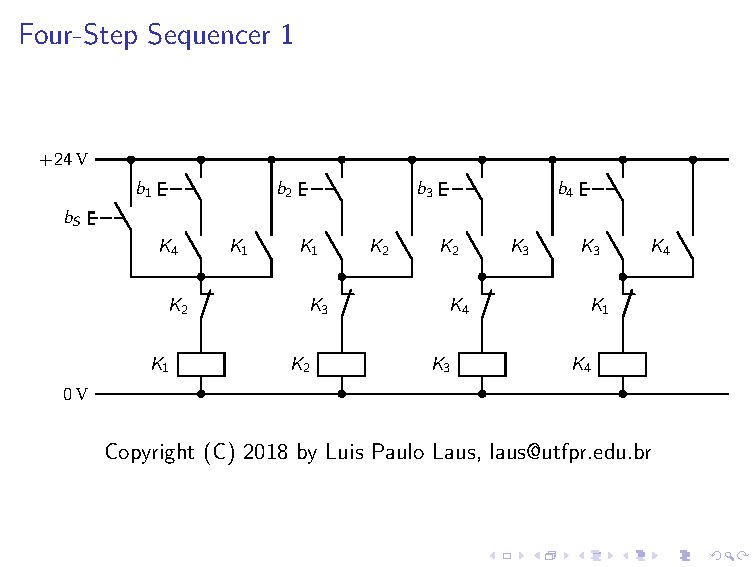
\includepdf[pages=-,offset=-116 285,noautoscale]{BeamerAnimation.pdf}

\end{document}